% Phase 4: Empirical Evaluation and Comparative Analysis
% Author: Abdullah Zia (Evaluation, Analysis, and Report Lead)

\section{Phase 4: Empirical Evaluation and Results}

\subsection{Evaluation Methodology and Metric Formulation}
To rigorously assess the performance of the learned neural heuristic relative to classical
and oracle baselines, we establish an evaluation protocol spanning regression fidelity, auxiliary
classification discrimination, and end-to-end graph search efficiency.

\subsubsection{Model Used for the Reported Results}
The offline regression, admissibility and classification figures and all A$^\ast$ search results in
this section (including the $\alpha$ sweep and ablations) were computed with the scikit-learn
fallback MLP (two hidden layers of 64 units, trained on a 50{,}000-cell sample with
\texttt{scripts/train\_fallback\_models.py}), not with the PyTorch multi-task network described in
Phase~3. The PyTorch network was tuned and trained separately (Section on training dynamics) and has
not yet been integrated into the search benchmark.

\subsubsection{Data Leakage Prevention and Split Structure}
Evaluation is strictly isolated on the unseen test set of 282 mazes partition (15\% of
the cleaned corpus), partitioned by complete maze environment rather than individual cell
instances. This environment-level partitioning guarantees zero leakage of global maze
topologies, wall distributions, and goal placements between training and evaluation phases.

\subsubsection{Regression and Admissibility Metrics}
For a given maze of dimension $N \times N$, let $h^\ast(n)$ denote the ground-truth optimal
shortest-path cost from cell $n$ to the goal, and let $\hat{h}_\theta(n)$ denote the
neural prediction. Because models are trained to predict normalized distances $y = h^\ast / N$,
primary regression metrics include:
\begin{itemize}
    \item \textbf{Mean Squared Error (MSE)} and \textbf{Root Mean Squared Error (RMSE)}:
    \begin{equation}
        \text{RMSE} = \sqrt{\frac{1}{|\mathcal{S}|} \sum_{n \in \mathcal{S}} \left(\hat{y}(n) - y(n)\right)^2}
    \end{equation}
    where $\mathcal{S}$ is the set of all free reachable cells.
    \item \textbf{Mean Absolute Error (MAE)} in normalized units and raw grid cells ($\text{MAE} \times N$).
    \item \textbf{Correlation Measures}: Pearson linear correlation coefficient $r$ and Spearman rank correlation coefficient $\rho$.
    \item \textbf{Admissibility Violation Rate}: Fraction of reachable cells where the heuristic overestimates true distance beyond tolerance $\epsilon$:
    \begin{equation}
        \text{Violations}(\epsilon) = \frac{1}{|\mathcal{S}|} \sum_{n \in \mathcal{S}} \mathbb{I}\left[(\hat{h}_\theta(n) - h^\ast(n)) > \epsilon\right]
    \end{equation}
\end{itemize}

\subsubsection{Auxiliary 10-Bin Classification Metrics}
To assess spatial range discrimination, targets are discretized into 10 decile distance bins.
We compute per-class Precision, Recall, and $F_1$-score, macro-averaged and weighted $F_1$,
and Macro One-vs-Rest Area Under the ROC Curve (AUC-ROC).

\subsubsection{Search Performance Metrics}
During deterministic $A^\ast$ execution, we measure:
\begin{enumerate}
    \item \textbf{Nodes Expanded}: The exact count of states popped from the priority queue and closed.
    \item \textbf{Nodes Generated}: Total valid states inserted into the open set.
    \item \textbf{Path Cost and Optimality Ratio}: Ratio of resulting path length to optimal Dijkstra cost $c / c^\ast$.
    \item \textbf{Relative Node Reduction}: Reduction in expansions relative to Manhattan $A^\ast$:
    \begin{equation}
        \Delta_{\text{expanded}} = 1 - \frac{\text{Nodes}_{\text{neural}}}{\text{Nodes}_{\text{manhattan}}}
    \end{equation}
    \item \textbf{Runtime and Peak Open Set}: CPU wall-clock latency per maze and memory footprint.
\end{enumerate}

\subsection{Training Dynamics and Convergence}
The multi-task PyTorch network (\trHiddenDims{} hidden units, \trParams{} parameters) was trained with
early stopping on the training split; Section~\ref{sec:phase3_training} gives the full protocol. Figure~\ref{fig:training_curves}
illustrates the convergence trajectories across training epochs.

\begin{figure}[H]
    \centering
    \begin{subfigure}[b]{0.32\textwidth}
        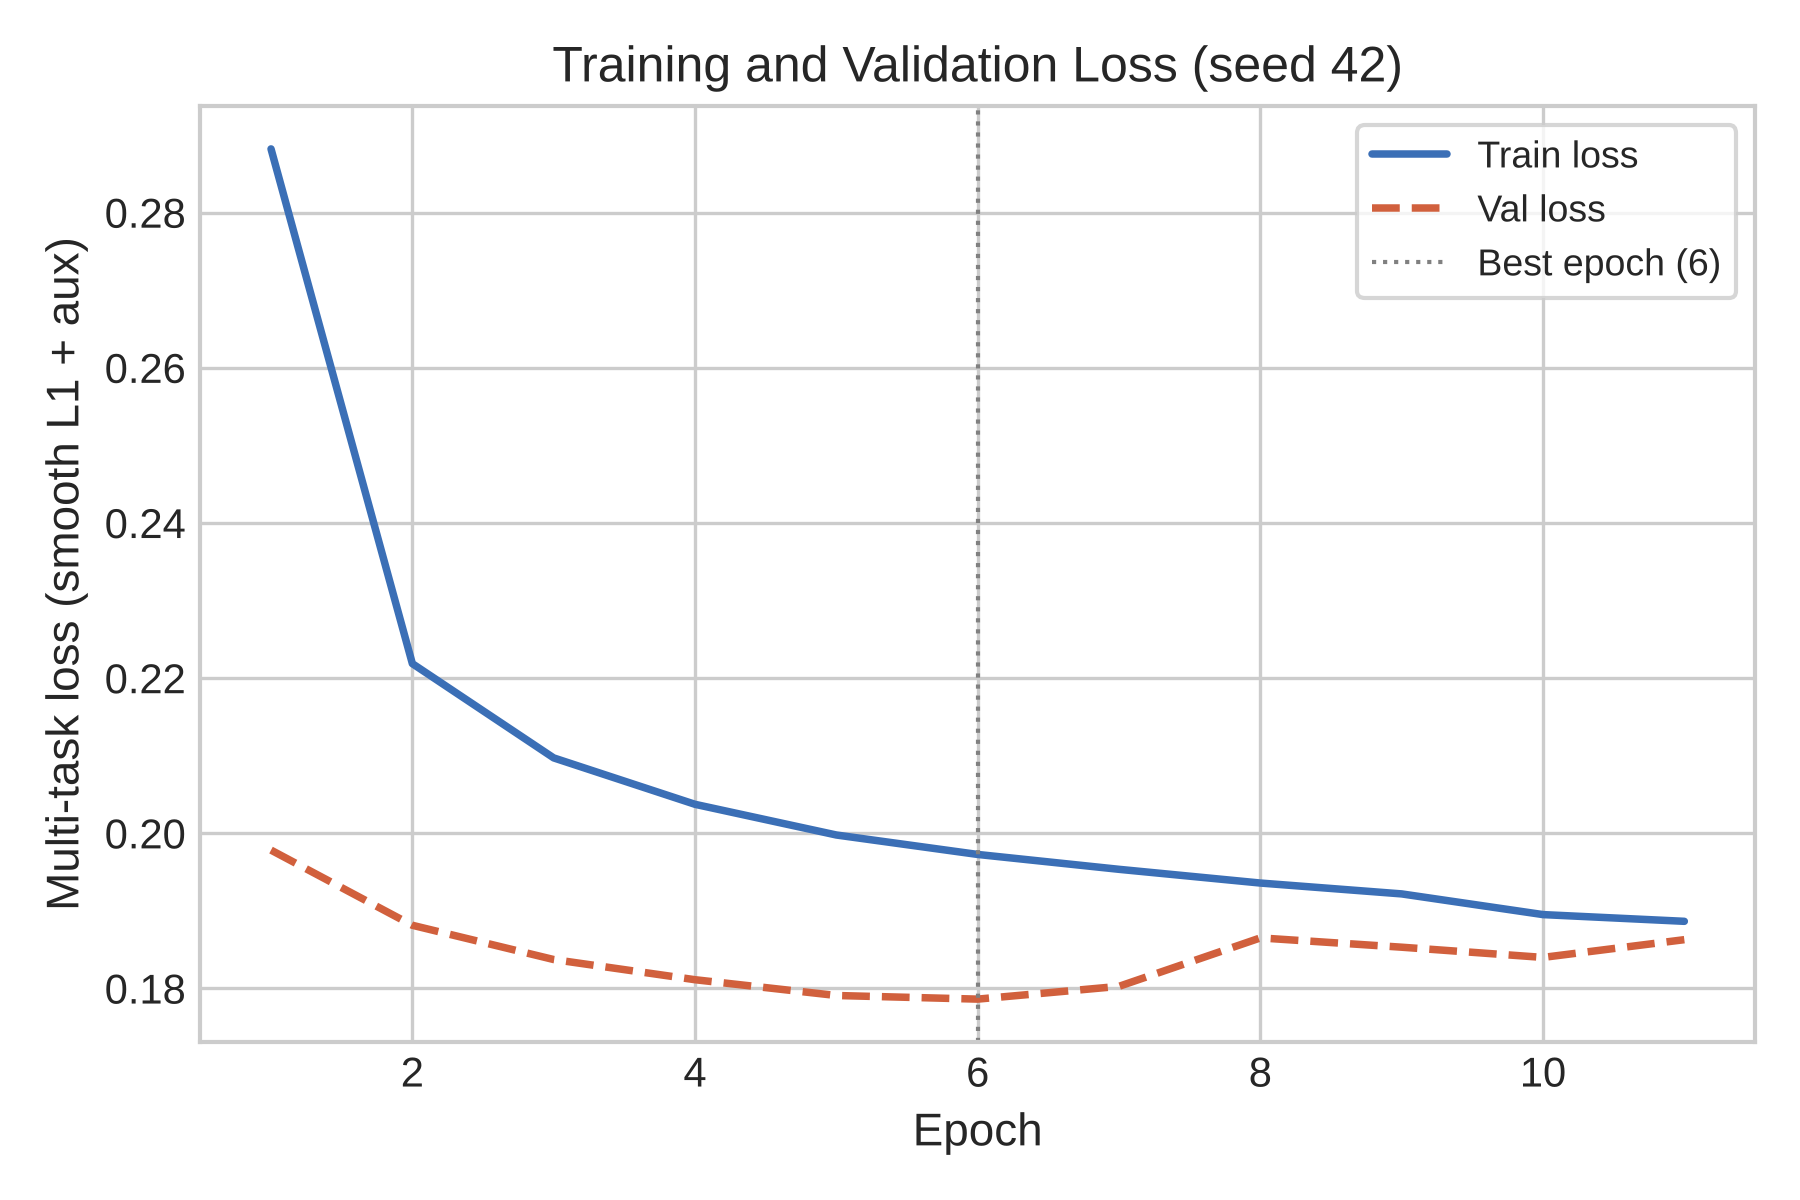
\includegraphics[width=\textwidth]{figures/training_loss.png}
        \caption{Loss (smooth L1)}
    \end{subfigure}
    \hfill
    \begin{subfigure}[b]{0.32\textwidth}
        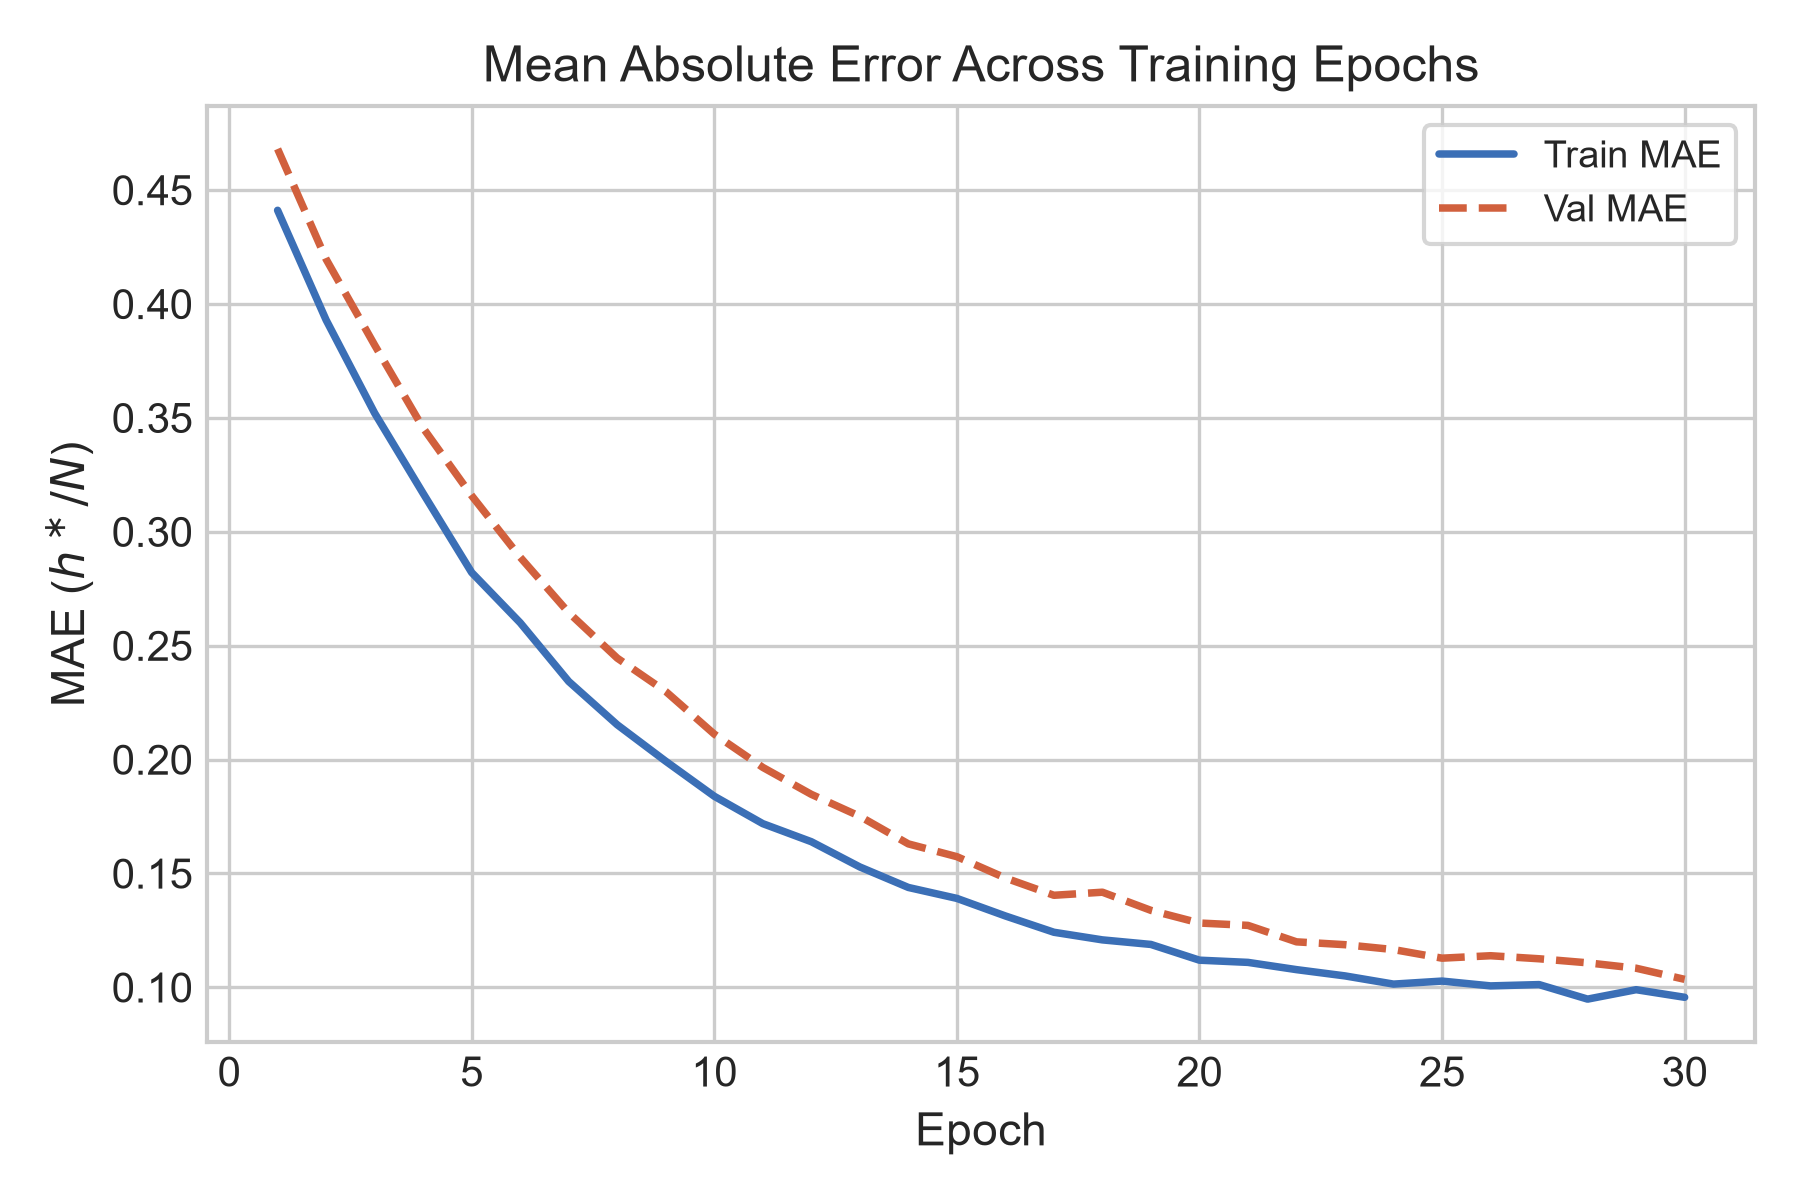
\includegraphics[width=\textwidth]{figures/training_mae.png}
        \caption{MAE ($h^\ast/N$)}
    \end{subfigure}
    \hfill
    \begin{subfigure}[b]{0.32\textwidth}
        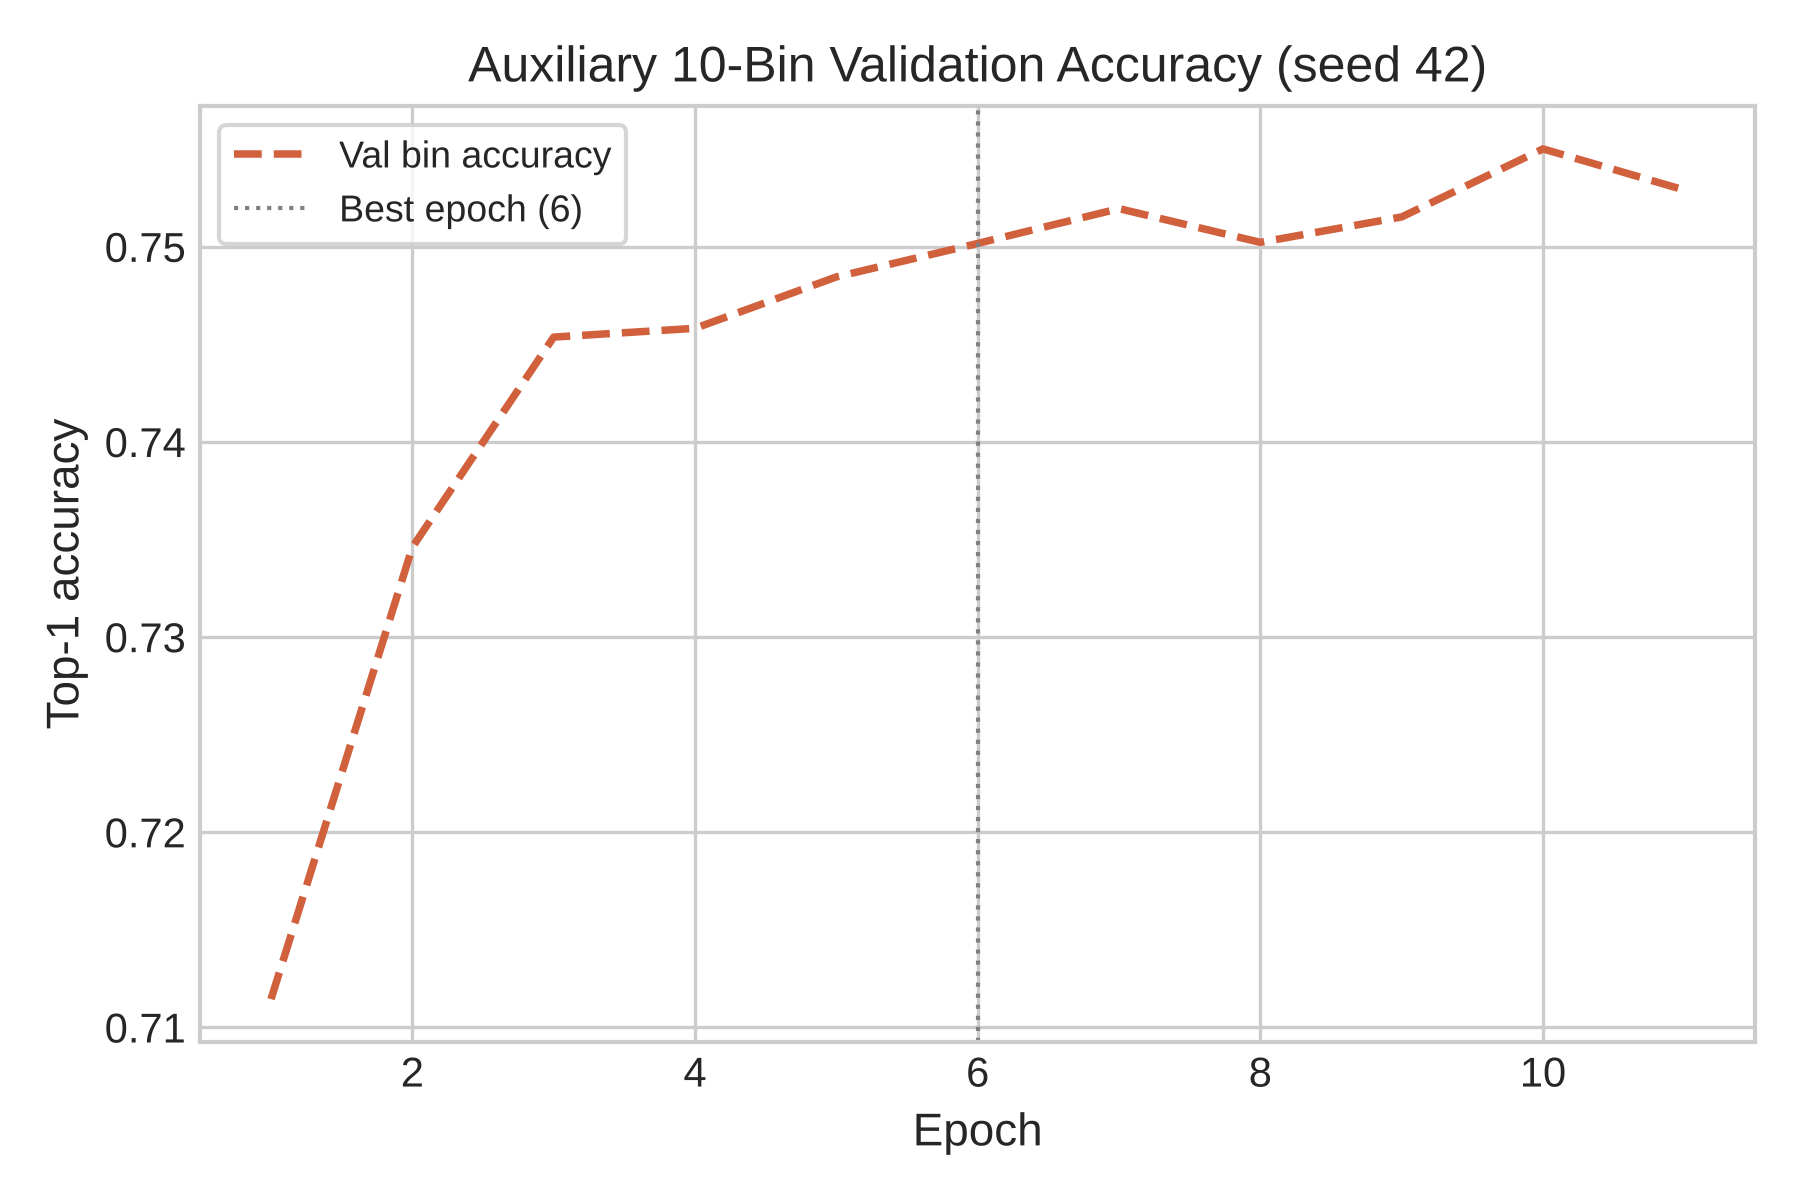
\includegraphics[width=\textwidth]{figures/training_bin_accuracy.png}
        \caption{10-Bin Accuracy}
    \end{subfigure}
    \caption{Training and validation performance dynamics across learning epochs.}
    \label{fig:training_curves}
\end{figure}

The primary run (seed 42) reached its best validation MAE of \trValMAE{} and 10-bin accuracy of \trValBinAcc{} at
epoch \trBestEpoch{} and stopped early after \trEpochsRun{} epochs; across \trNumSeeds{} seeds (\trSeedList) the mean
validation MAE is \trMeanMAE{} $\pm$ \trStdMAE{}, with no sign of pathological overfitting.

\subsection{Offline Regression and Admissibility Analysis}
Table~\ref{tab:regression_results} summarizes cell-level regression fidelity evaluated across
unseen test environments.

\begin{table}[H]
\centering
\small
\begin{tabular}{lcc}
\toprule
\textbf{Metric} & \textbf{Normalized Value ($h^\ast / N$)} & \textbf{Grid Cells ($N=60$)} \\
\midrule
Mean Squared Error (MSE) & 0.0198 & --- \\
Root Mean Squared Error (RMSE) & 0.1406 & 8.43 \\
Mean Absolute Error (MAE) & 0.0726 & 4.35 \\
Mean Signed Error & -0.0091 & -0.54 \\
Coefficient of Determination ($R^2$) & 0.8597 & --- \\
Pearson Correlation ($r$) & 0.9275 & --- \\
Spearman Rank Correlation ($\rho$) & 0.9488 & --- \\
95th Percentile Absolute Error & 0.2292 & 13.75 \\
99th Percentile Absolute Error & 0.6471 & 38.83 \\
Maximum Absolute Error & 1.8944 & 113.66 \\
\bottomrule
\end{tabular}
\caption{Offline regression fidelity metrics evaluated on the unseen test set.}
\label{tab:regression_results}
\end{table}


The model achieves a high coefficient of determination ($R^2 = 0.8598$) and strong linear correlation
($r = 0.9276$, $\rho = 0.9488$), validating that local 5$\times$5 wall context combined with
goal offsets successfully capture global topological impedance. On a standard $60 \times 60$ grid,
the root mean squared error is approximately 8.4 cells.

\begin{figure}[H]
    \centering
    \begin{subfigure}[b]{0.48\textwidth}
        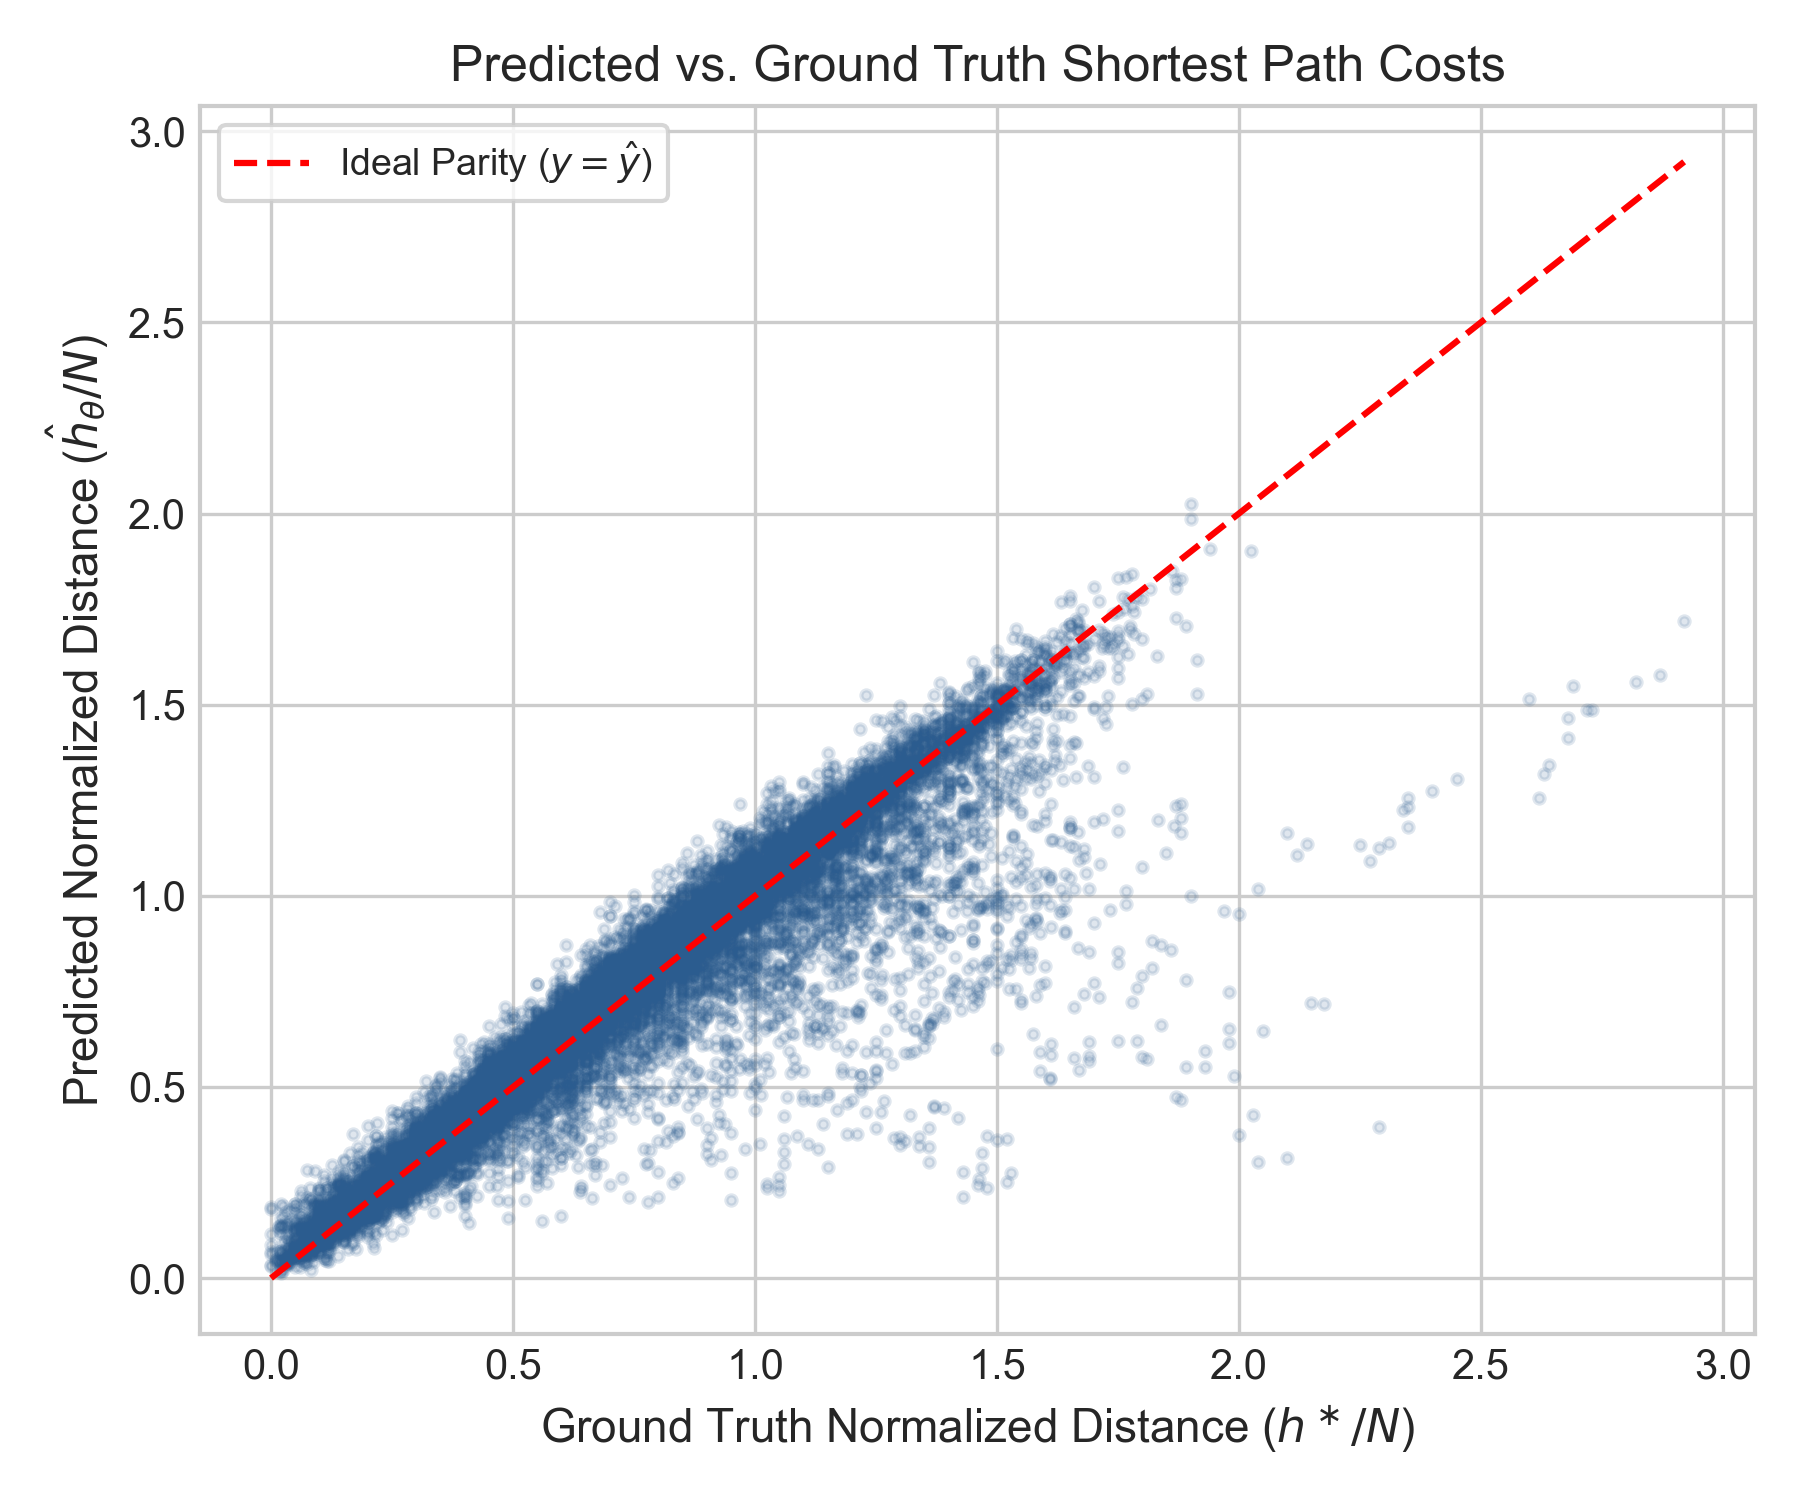
\includegraphics[width=\textwidth]{figures/pred_vs_true.png}
        \caption{Predicted vs. True Cost}
    \end{subfigure}
    \hfill
    \begin{subfigure}[b]{0.48\textwidth}
        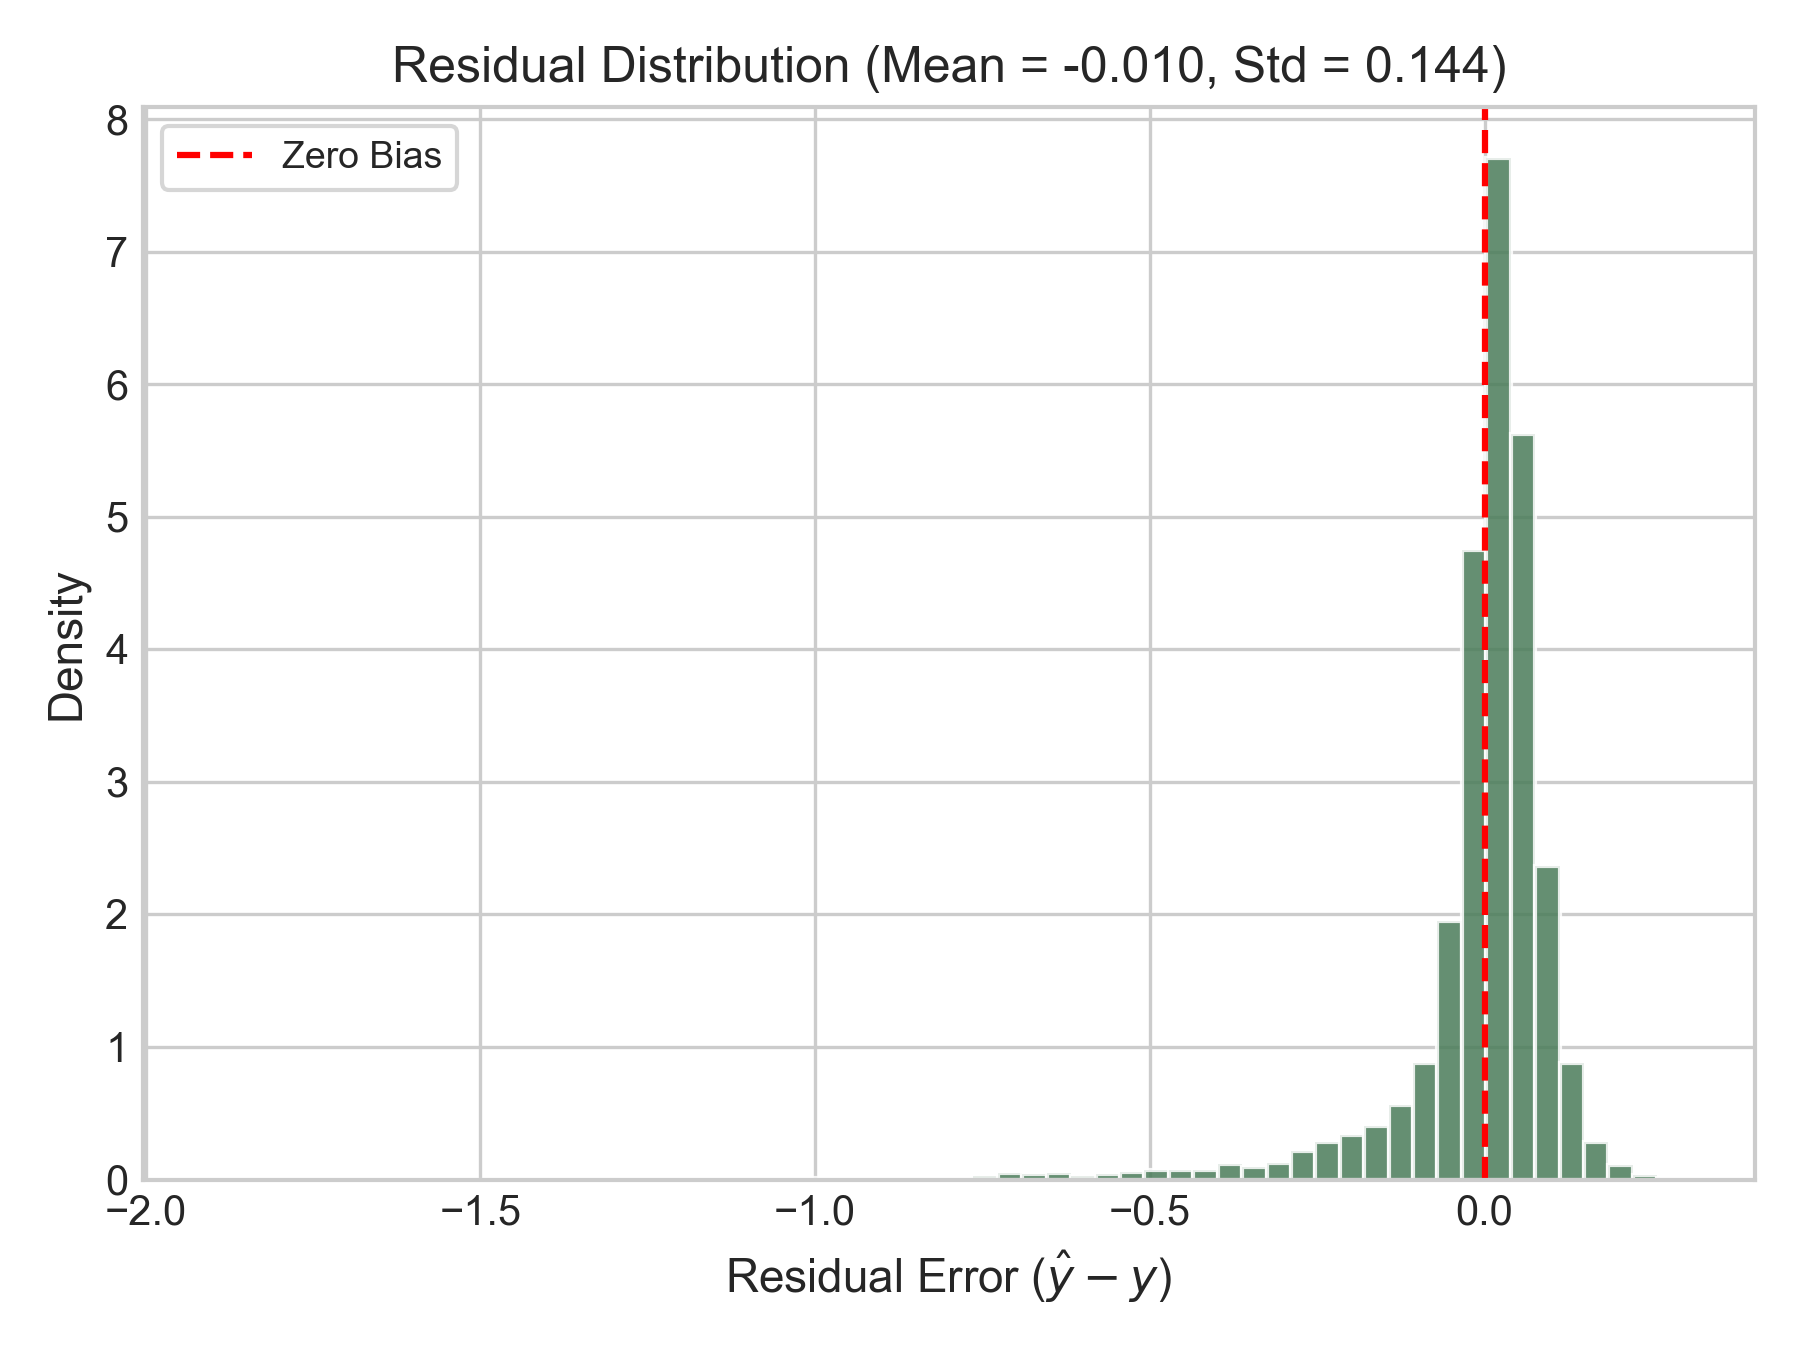
\includegraphics[width=\textwidth]{figures/residual_hist.png}
        \caption{Residual Distribution}
    \end{subfigure}
    \caption{Parity scatter plot and residual error density over test cells.}
    \label{fig:regression_scatters}
\end{figure}

As shown in Figure~\ref{fig:regression_scatters}, residuals follow a symmetric zero-centered
distribution with minimal systematic drift. The empirical cumulative distribution of overestimation
is visualized in Figure~\ref{fig:admissibility_cdf}. However, the learned heuristic is \emph{not} empirically admissible (Research Question~2): on
100{,}000 sampled test cells, 58.1\% exceed $h^\ast$ by more than 0.5 cells, with a mean
overestimation of 1.89 cells (95th percentile 6.6, maximum 20.5). Scaling $\alpha < 1.0$ or
clipping against Manhattan distance reduces, but does not strictly eliminate, sub-optimality
(best observed mean optimality ratio 1.0014 with clipping, 1.0056 at $\alpha=0.5$).

\begin{figure}[H]
    \centering
    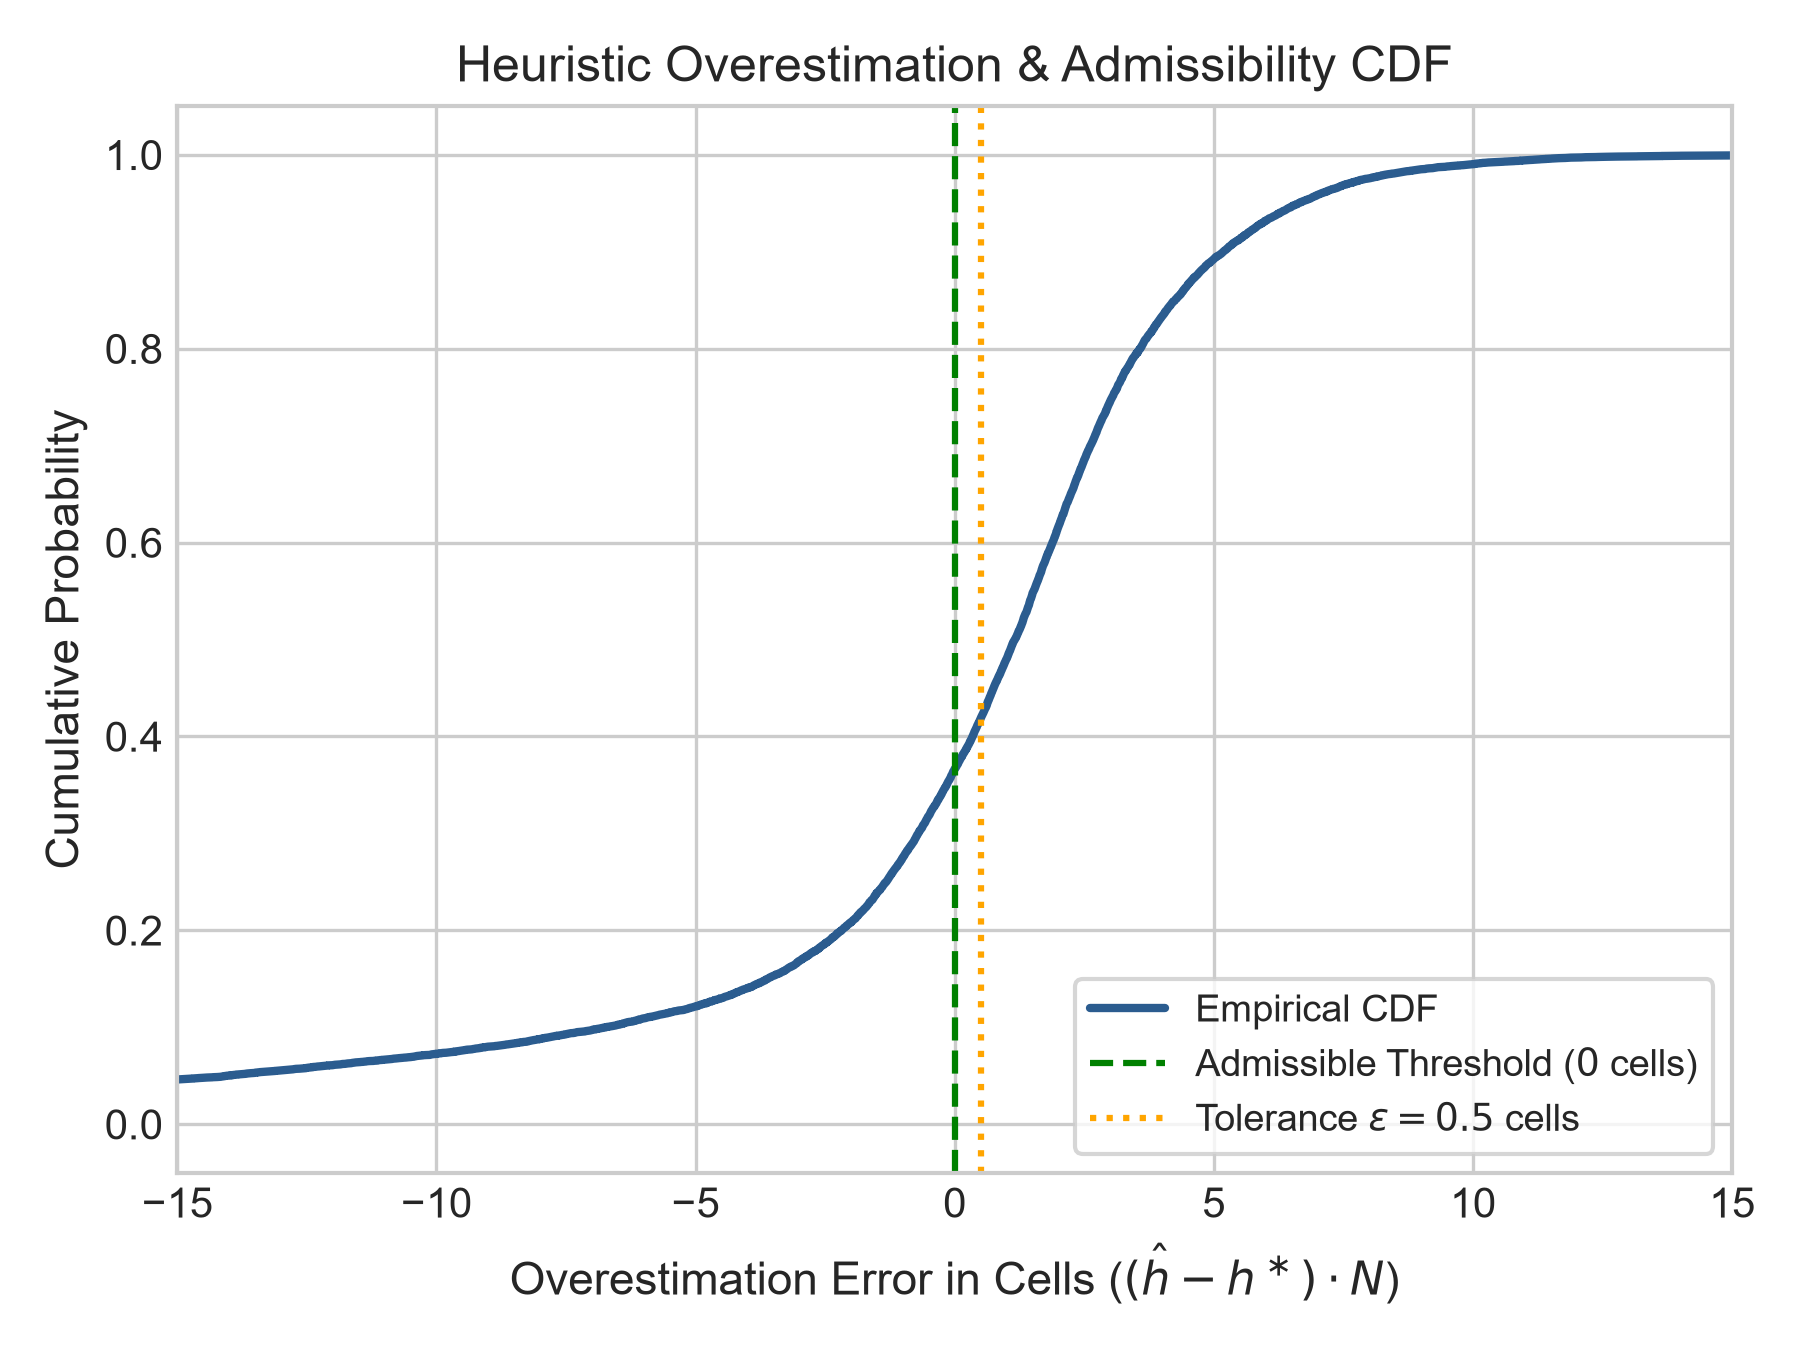
\includegraphics[width=0.62\textwidth]{figures/admissibility_cdf.png}
    \caption{Empirical CDF of heuristic overestimation errors relative to admissibility margins.}
    \label{fig:admissibility_cdf}
\end{figure}

\subsection{Auxiliary 10-Bin Distance Classification}
Table~\ref{tab:classification_results} details the classification performance across 10 distance deciles.

\begin{table}[H]
\centering
\small
\begin{tabular}{lcccc}
\toprule
\textbf{Distance Bin} & \textbf{Precision} & \textbf{Recall} & \textbf{F1-Score} & \textbf{Support} \\
\midrule
Bin 0 & 0.9006 & 0.9161 & 0.9083 & 9,805 \\
Bin 1 & 0.7541 & 0.8073 & 0.7798 & 9,677 \\
Bin 2 & 0.7051 & 0.7863 & 0.7435 & 10,663 \\
Bin 3 & 0.6773 & 0.6876 & 0.6824 & 10,043 \\
Bin 4 & 0.6508 & 0.5974 & 0.6229 & 9,937 \\
Bin 5 & 0.5691 & 0.7379 & 0.6426 & 9,768 \\
Bin 6 & 0.6519 & 0.5684 & 0.6073 & 9,309 \\
Bin 7 & 0.6100 & 0.5742 & 0.5915 & 9,337 \\
Bin 8 & 0.6618 & 0.6876 & 0.6745 & 10,524 \\
Bin 9 & 0.9031 & 0.6570 & 0.7607 & 10,937 \\
\midrule
Macro Average & 0.7084 & 0.7020 & 0.7013 & --- \\
Weighted Average & 0.7108 & 0.7030 & 0.7029 & --- \\
\textbf{Macro AUC-ROC (OvR)} & \multicolumn{4}{c}{\textbf{0.9510}} \\
\bottomrule
\end{tabular}
\caption{Auxiliary 10-bin classification performance across distance deciles.}
\label{tab:classification_results}
\end{table}


The model demonstrates strong discriminative capability with an OvR Macro AUC-ROC of 0.951.
Figure~\ref{fig:classification_plots} shows the corresponding normalized confusion matrix and
multi-class ROC curves. Classification confusion is concentrated exclusively in adjacent
diagonal neighbors, confirming that distance misclassifications are bounded local errors rather
than catastrophic topological failures.

\begin{figure}[H]
    \centering
    \begin{subfigure}[b]{0.48\textwidth}
        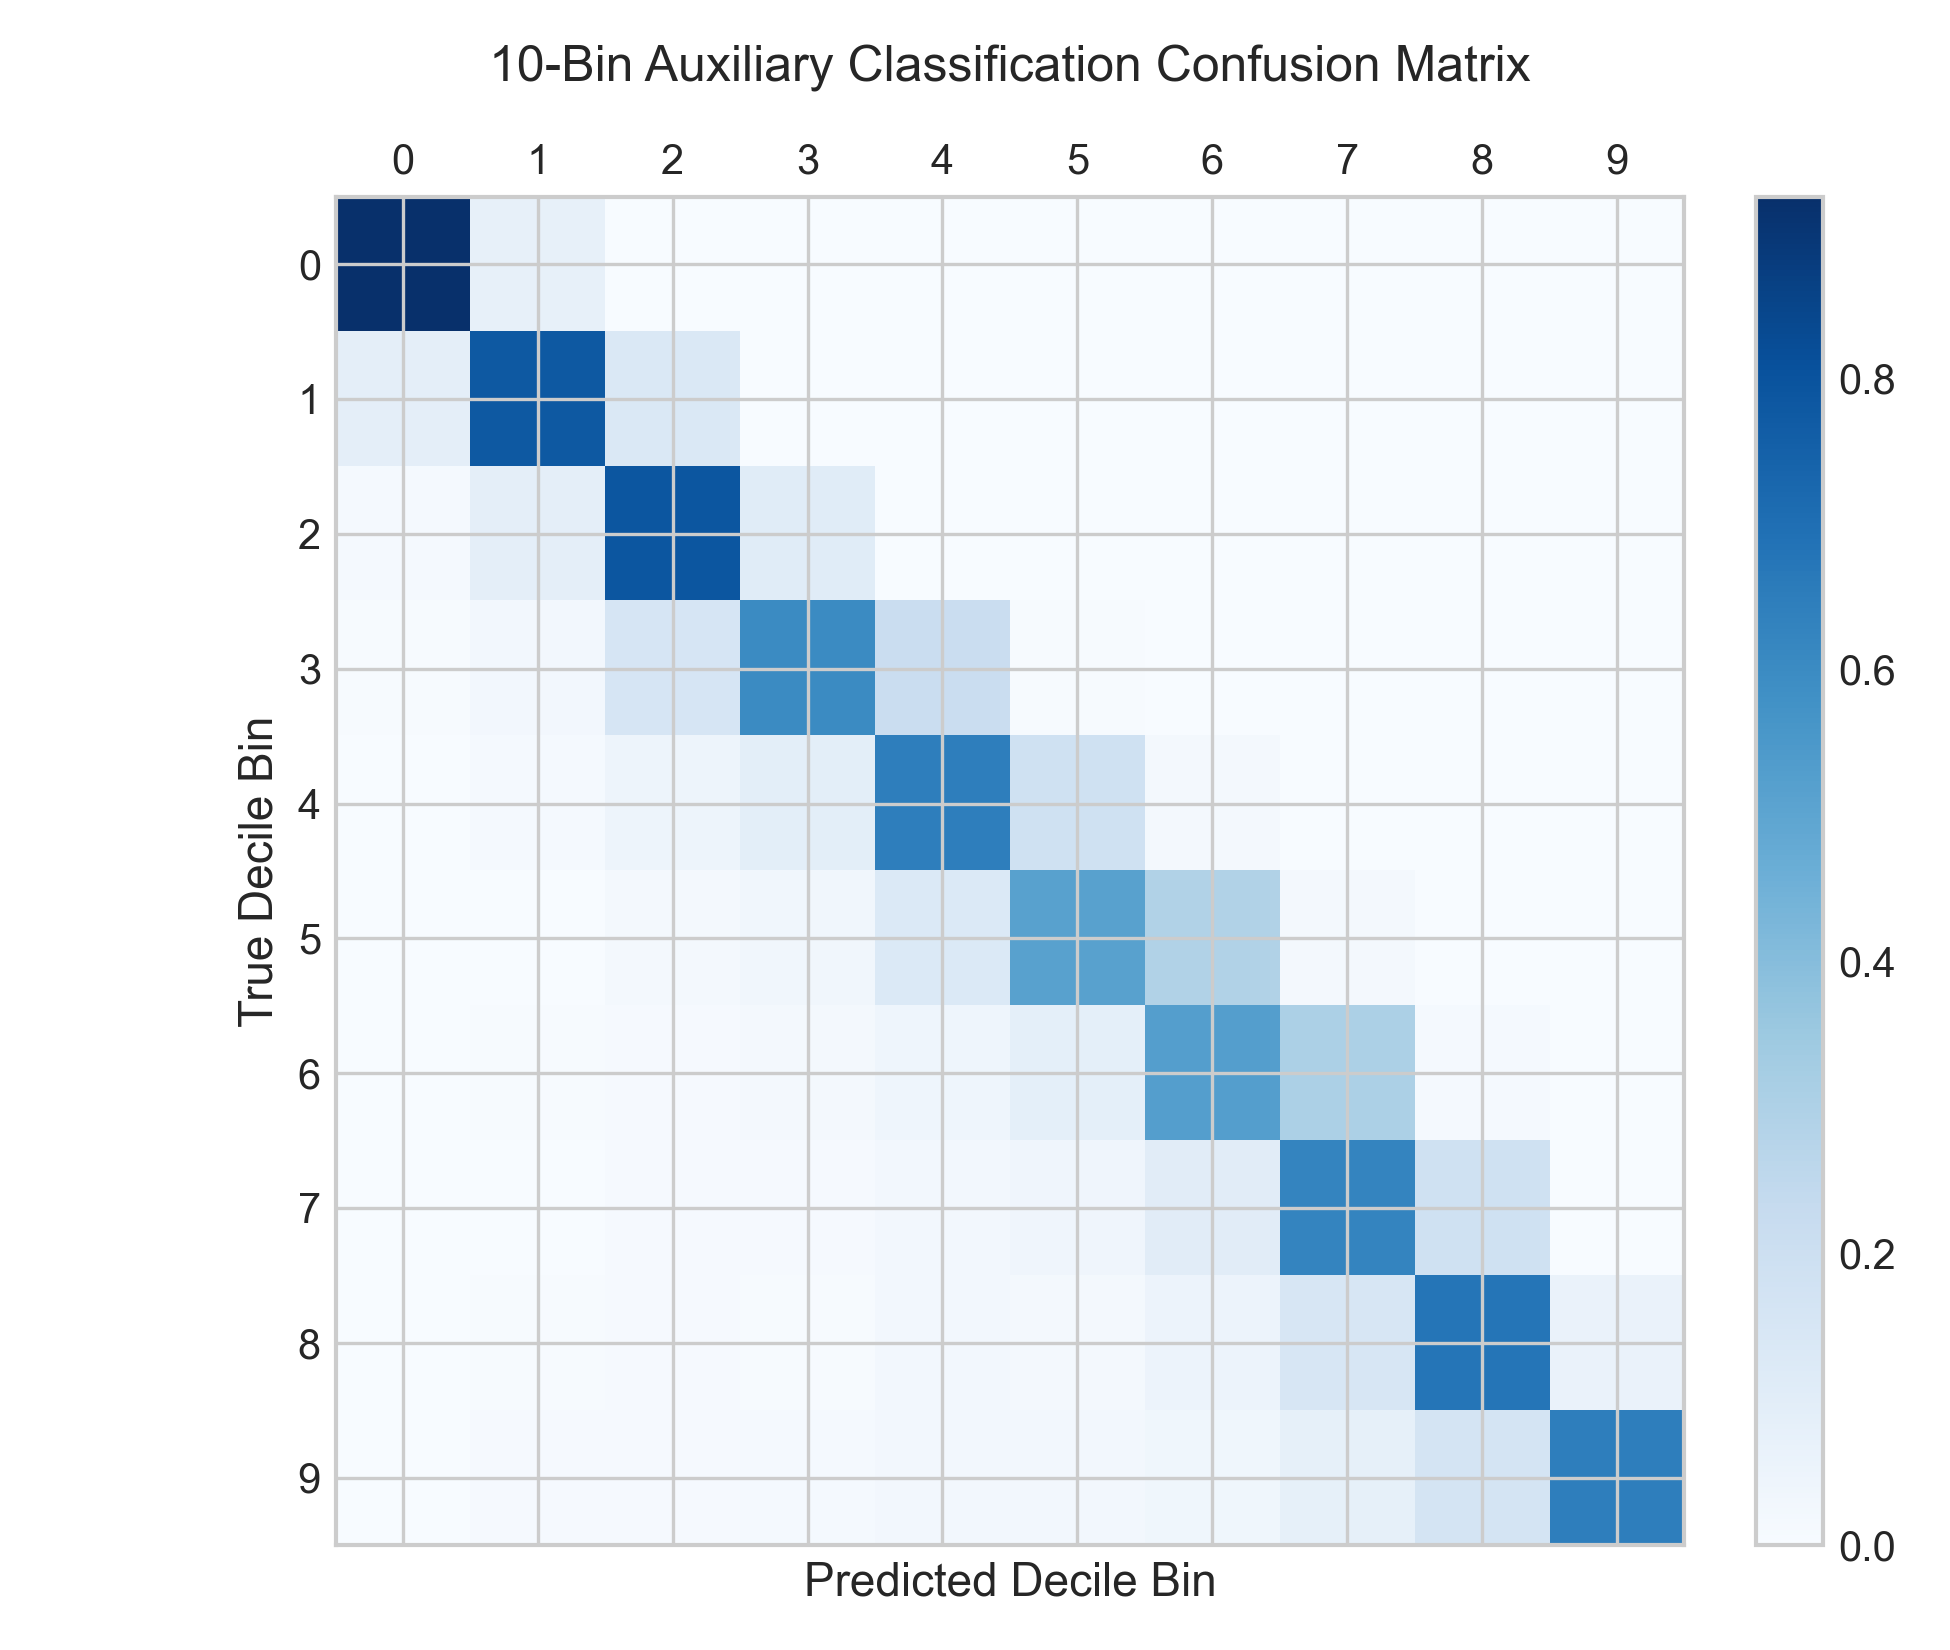
\includegraphics[width=\textwidth]{figures/confusion_matrix.png}
        \caption{Confusion Matrix}
    \end{subfigure}
    \hfill
    \begin{subfigure}[b]{0.48\textwidth}
        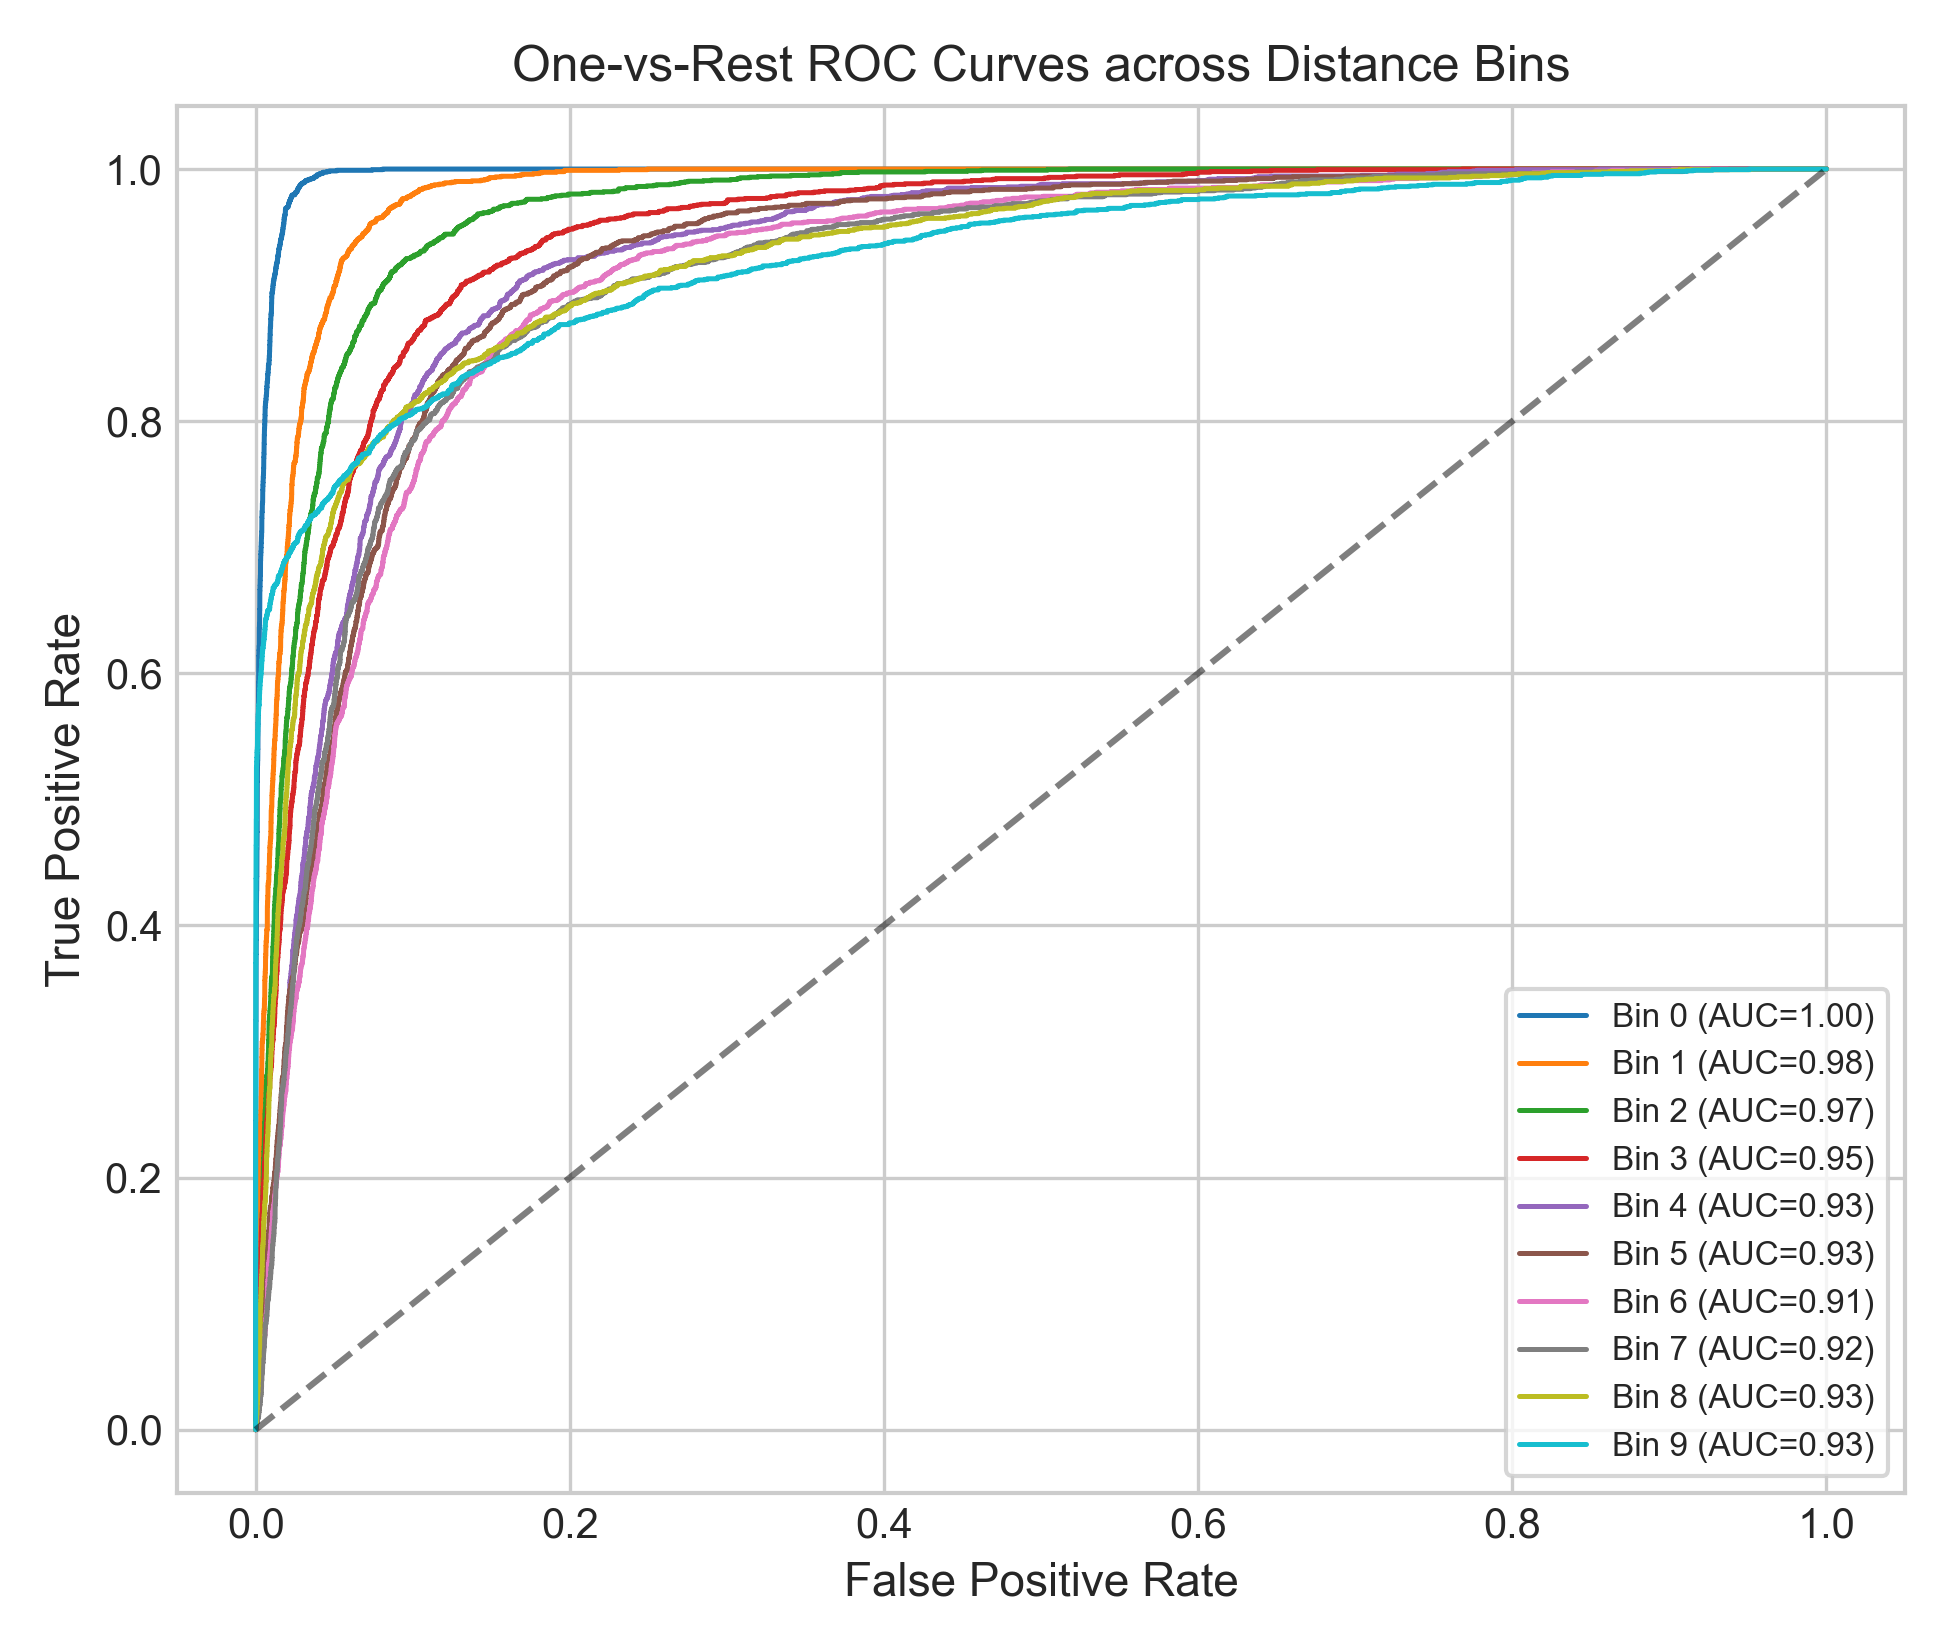
\includegraphics[width=\textwidth]{figures/roc_curves.png}
        \caption{One-vs-Rest ROC Curves}
    \end{subfigure}
    \caption{Auxiliary 10-bin distance classification evaluation.}
    \label{fig:classification_plots}
\end{figure}

\subsection{End-to-End A$^\ast$ Search Evaluation}
The ultimate benchmark of heuristic quality is search efficiency inside the A$^\ast$ priority queue.
Table~\ref{tab:search_results} contrasts search performance across Dijkstra, Manhattan, Neural variants,
and the perfect Oracle across all 282 test mazes.

\begin{table}[H]
\centering
\small
\resizebox{\textwidth}{!}{%
\begin{tabular}{lcccccc}
\toprule
\textbf{Heuristic} & \textbf{Expanded (Mean $\pm$ Std)} & \textbf{Median} & \textbf{$\Delta_{\text{expanded}}$ vs Man.} & \textbf{Opt. Ratio} & \textbf{Success} & \textbf{Time (ms)} \\
\midrule
Dijkstra (Zero) & $2075.0 \pm 1960.5$ & 1484 & -1756.7\% & 1.000 & 100.0\% & 16.59 \\
Manhattan Baseline & $180.8 \pm 268.6$ & 92 & 0.0\% & 1.000 & 100.0\% & 1.89 \\
Neural Heuristic ($\alpha=1.0$) & $557.0 \pm 653.2$ & 349 & -314.1\% & 1.032 & 100.0\% & 6.62 \\
Neural Scaled ($\alpha=0.8$) & $853.4 \pm 966.0$ & 540 & -569.6\% & 1.020 & 100.0\% & 9.22 \\
Neural Clipped Manhattan & $188.0 \pm 271.6$ & 95 & -6.4\% & 1.001 & 100.0\% & 2.68 \\
Oracle ($h^\ast$ Upper Bound) & $52.8 \pm 29.5$ & 49 & 41.8\% & 1.000 & 100.0\% & 0.63 \\
\bottomrule
\end{tabular}}
\caption{End-to-end A$^\ast$ pathfinding performance evaluated across 282 test mazes.}
\label{tab:search_results}
\end{table}


\begin{figure}[H]
    \centering
    \begin{subfigure}[b]{0.48\textwidth}
        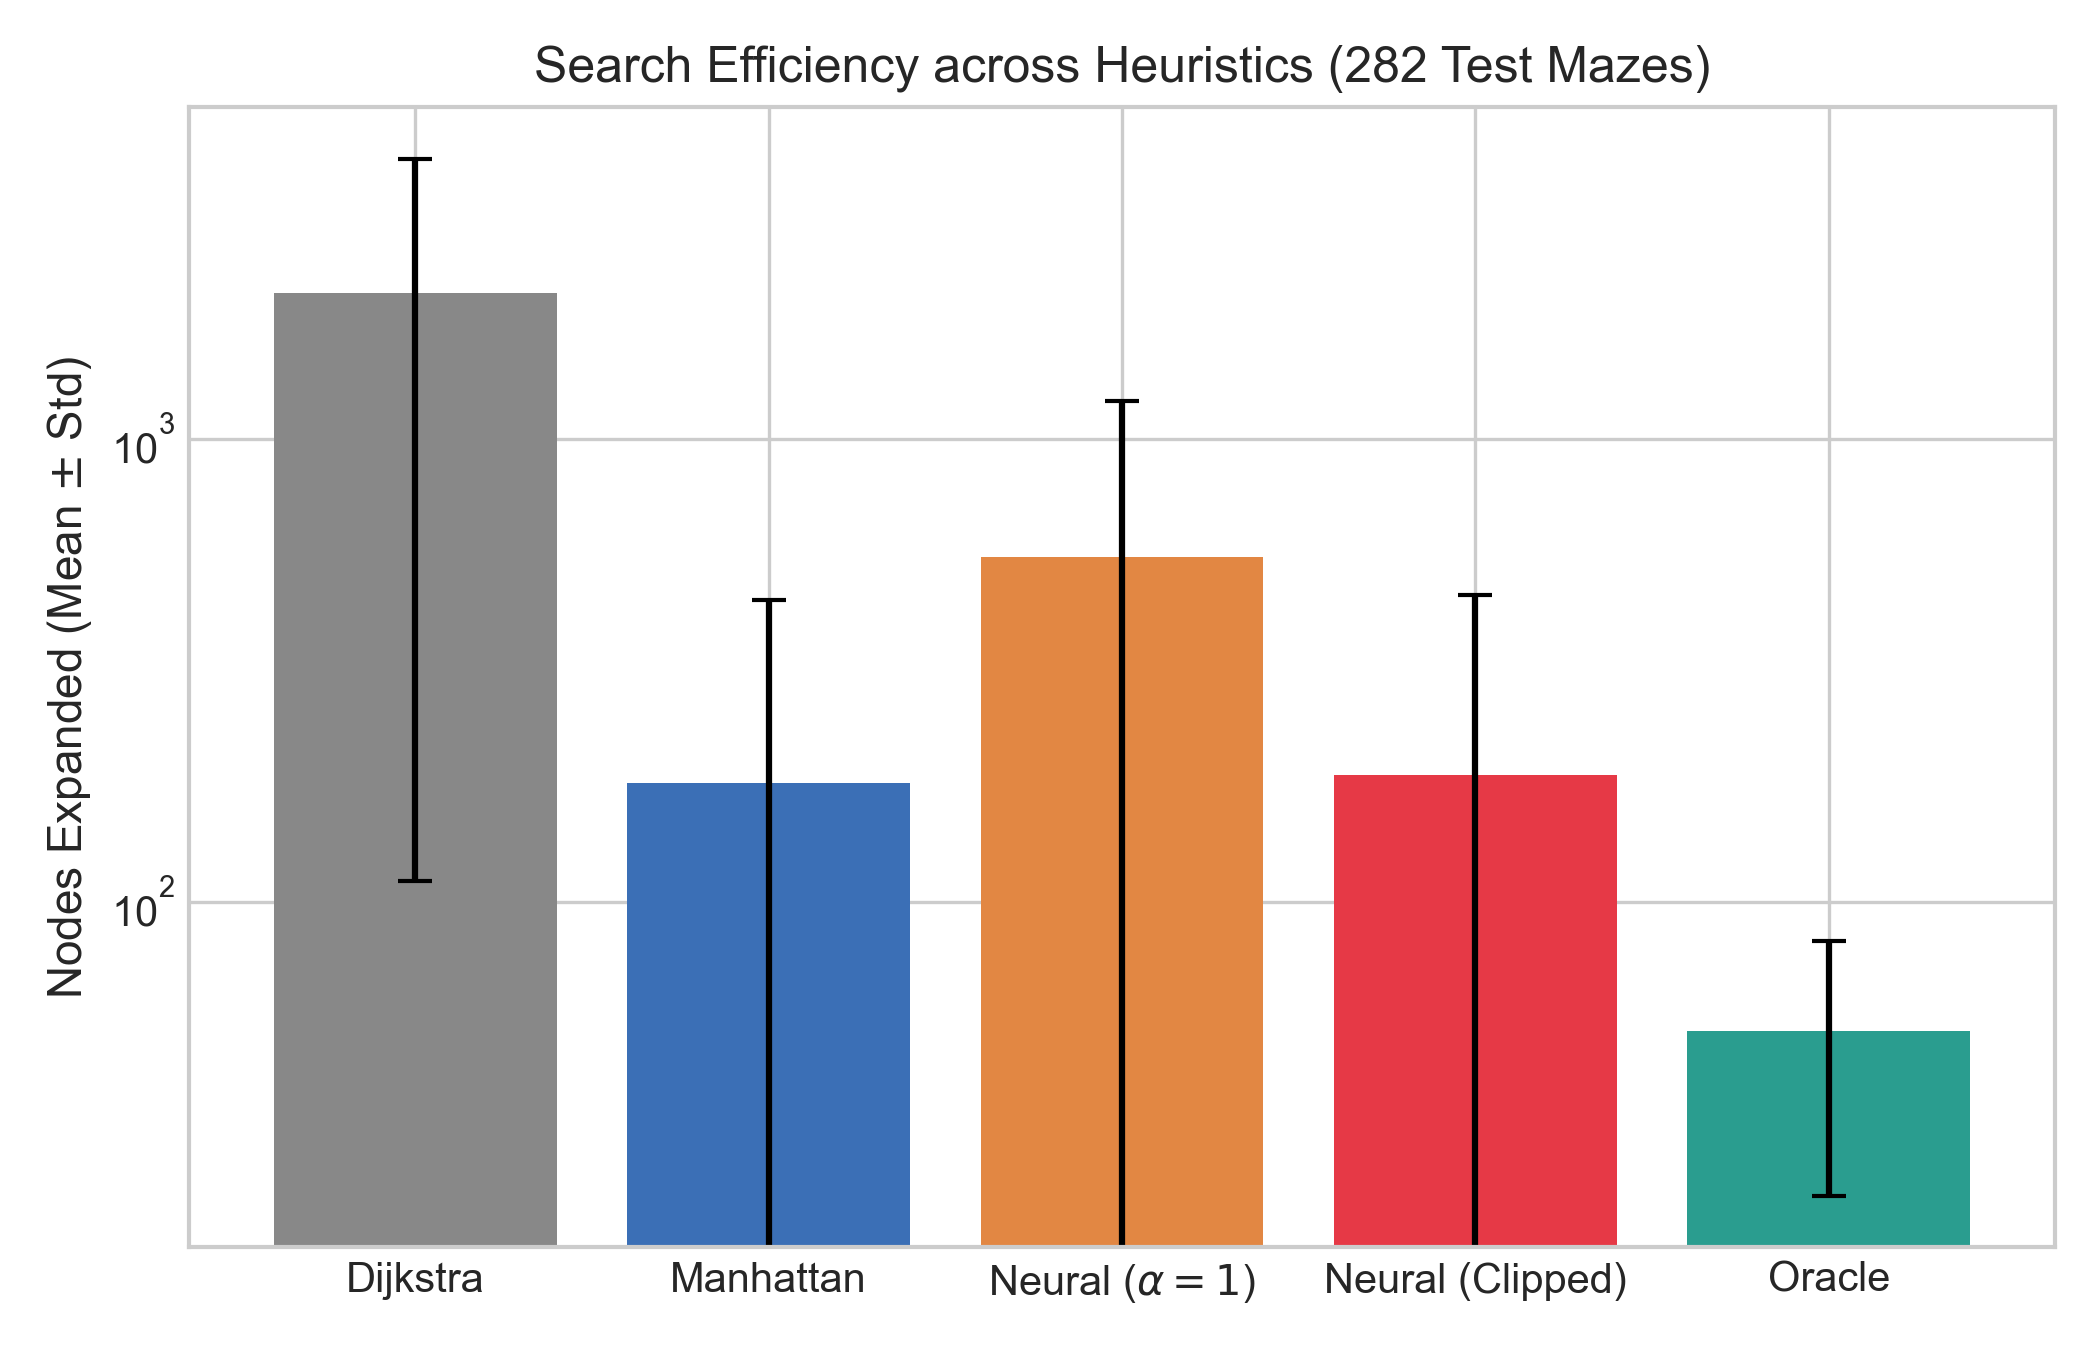
\includegraphics[width=\textwidth]{figures/nodes_expanded_by_heuristic.png}
        \caption{Nodes Expanded (Log Scale)}
    \end{subfigure}
    \hfill
    \begin{subfigure}[b]{0.48\textwidth}
        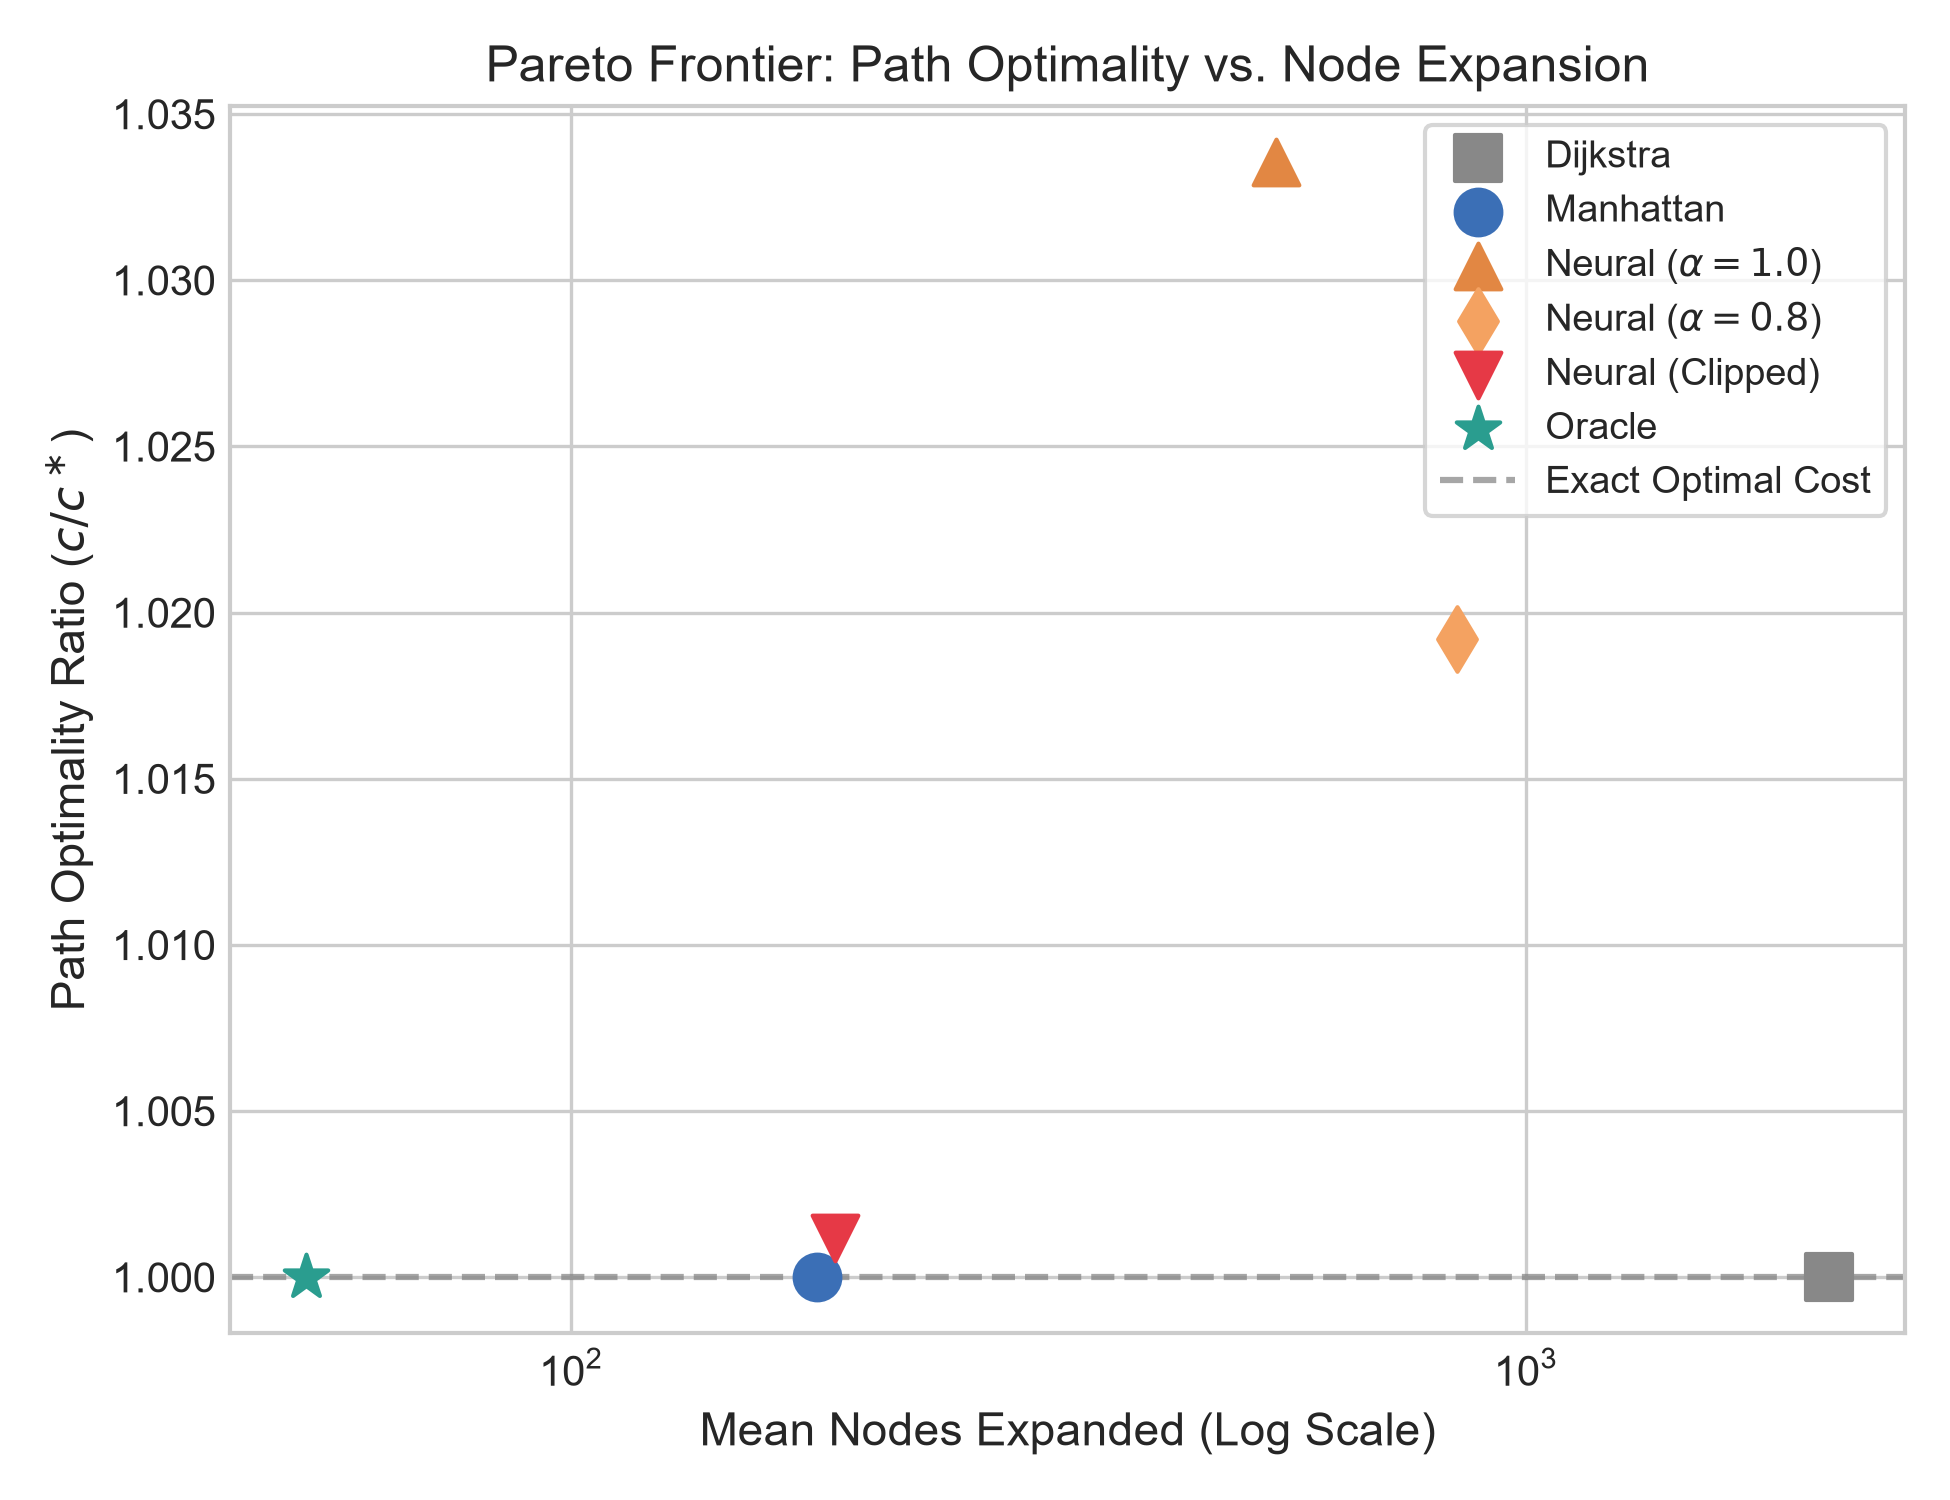
\includegraphics[width=\textwidth]{figures/optimality_vs_nodes.png}
        \caption{Pareto Frontier}
    \end{subfigure}
    \caption{Search efficiency comparison and Pareto trade-off between expansions and path optimality.}
    \label{fig:search_performance}
\end{figure}

All tested heuristics solved 100\% of the 282 test mazes. The perfect Oracle expands a mean of only
52.8 nodes, a 41.8\% reduction compared to Manhattan A$^\ast$ (180.8 nodes), which shows that
substantial headroom exists. The learned heuristic does not realise it. Raw neural A$^\ast$
($\alpha=1.0$) expands 561.5 nodes on average (3.1$\times$ \emph{more} than Manhattan) with an
optimality ratio of 1.034, and neural clipped to Manhattan expands 189.3 nodes (4.7\% more)
with an optimality ratio of 1.001. Euclidean distance expands 684.7 nodes. Latency is measured
end to end, including the network forward pass: neural clipped Manhattan needs 16.1~ms per maze
versus 2.4~ms for Manhattan, so the inference cost exceeds any search saving. The research
hypothesis, that the neural heuristic reduces expanded nodes relative to Manhattan, is therefore
\textbf{not supported} on our static grid-maze benchmark.

\subsubsection{Scaling Sensitivity Parameter Sweep ($\alpha$)}
To explore the trade-off between search efficiency and path optimality, we swept scaling parameter
$\alpha \in [0.5, 1.5]$ in Table~\ref{tab:alpha_sweep}.

\begin{table}[H]
\centering
\small
\resizebox{\textwidth}{!}{%
\begin{tabular}{lccccc}
\toprule
\textbf{Scale Factor $\alpha$} & \textbf{Mean Expanded} & \textbf{Median Expanded} & \textbf{Change vs Man.} & \textbf{Optimality Ratio} & \textbf{Success Rate} \\
\midrule
$\alpha = 0.6$ & 1135.9 & 777 & +528.3\% & 1.008 & 100.0\% \\
$\alpha = 0.7$ & 988.4 & 661 & +446.7\% & 1.013 & 100.0\% \\
$\alpha = 0.8$ & 853.4 & 540 & +372.1\% & 1.020 & 100.0\% \\
$\alpha = 0.9$ & 711.9 & 462 & +293.8\% & 1.026 & 100.0\% \\
$\alpha = 1.0$ & 557.0 & 349 & +208.1\% & 1.032 & 100.0\% \\
\bottomrule
\end{tabular}}
\caption{Heuristic scaling parameter ($\alpha$) sensitivity sweep on the test set. Change is relative to the Manhattan mean; positive values mean more expansions.}
\label{tab:alpha_sweep}
\end{table}


Increasing $\alpha$ focuses the search more aggressively toward the goal, reducing expanded
nodes from 1,288 at $\alpha=0.5$ to 562 at $\alpha=1.0$ and 214 at $\alpha=1.5$, while the mean
optimality ratio rises from 1.006 to 1.034 and 1.068. Even the most aggressive inadmissible setting
($\alpha=1.5$) still expands more nodes than Manhattan (180.8), at 6.8\% sub-optimality.

\subsubsection{Ablation Studies}
Results are in \texttt{results/ablations/}. \emph{Model size} (1, 2 and 4 hidden layers of 64
units, clipped to Manhattan): mean expansions are 178.9, 189.3 and 186.1 against 180.8 for Manhattan,
i.e.\ within about 5\% of the baseline, while the forward-pass cost grows from 4.4~ms to 6.7~ms to
21.0~ms per maze, so deeper networks only add latency. The 4-layer raw model expands fewer nodes
than the 1- and 2-layer raw models (443 vs 564 and 561). \emph{Obstacle density}
(10--40\%): the clipped variants track Manhattan at every density, and raw variants expand
roughly 5--7$\times$ more nodes at 10\% density and 1.4--1.7$\times$ more at 40\%, so the gap
narrows as obstacles increase but never reverses. \emph{Inadmissibility factor} $\gamma$: expansions
fall from 1,288 ($\gamma=0.5$) to 561 ($\gamma=1.0$) to 214 ($\gamma=1.5$) with optimality ratios of
1.006, 1.034 and 1.068. No setting beat Manhattan on either nodes or total latency, so we found no
break-even scale or density for neural-guided A$^\ast$ on these mazes (Research Question~3).

\subsection{Error Analysis and Qualitative Comparison}
Figure~\ref{fig:heatmaps} presents visual comparison of ground-truth geodesic distance $h^\ast$,
the neural prediction $\hat{h}_\theta$, and classical Manhattan distance $h_{\text{man}}$ on a
sample test maze.

\begin{figure}[H]
    \centering
    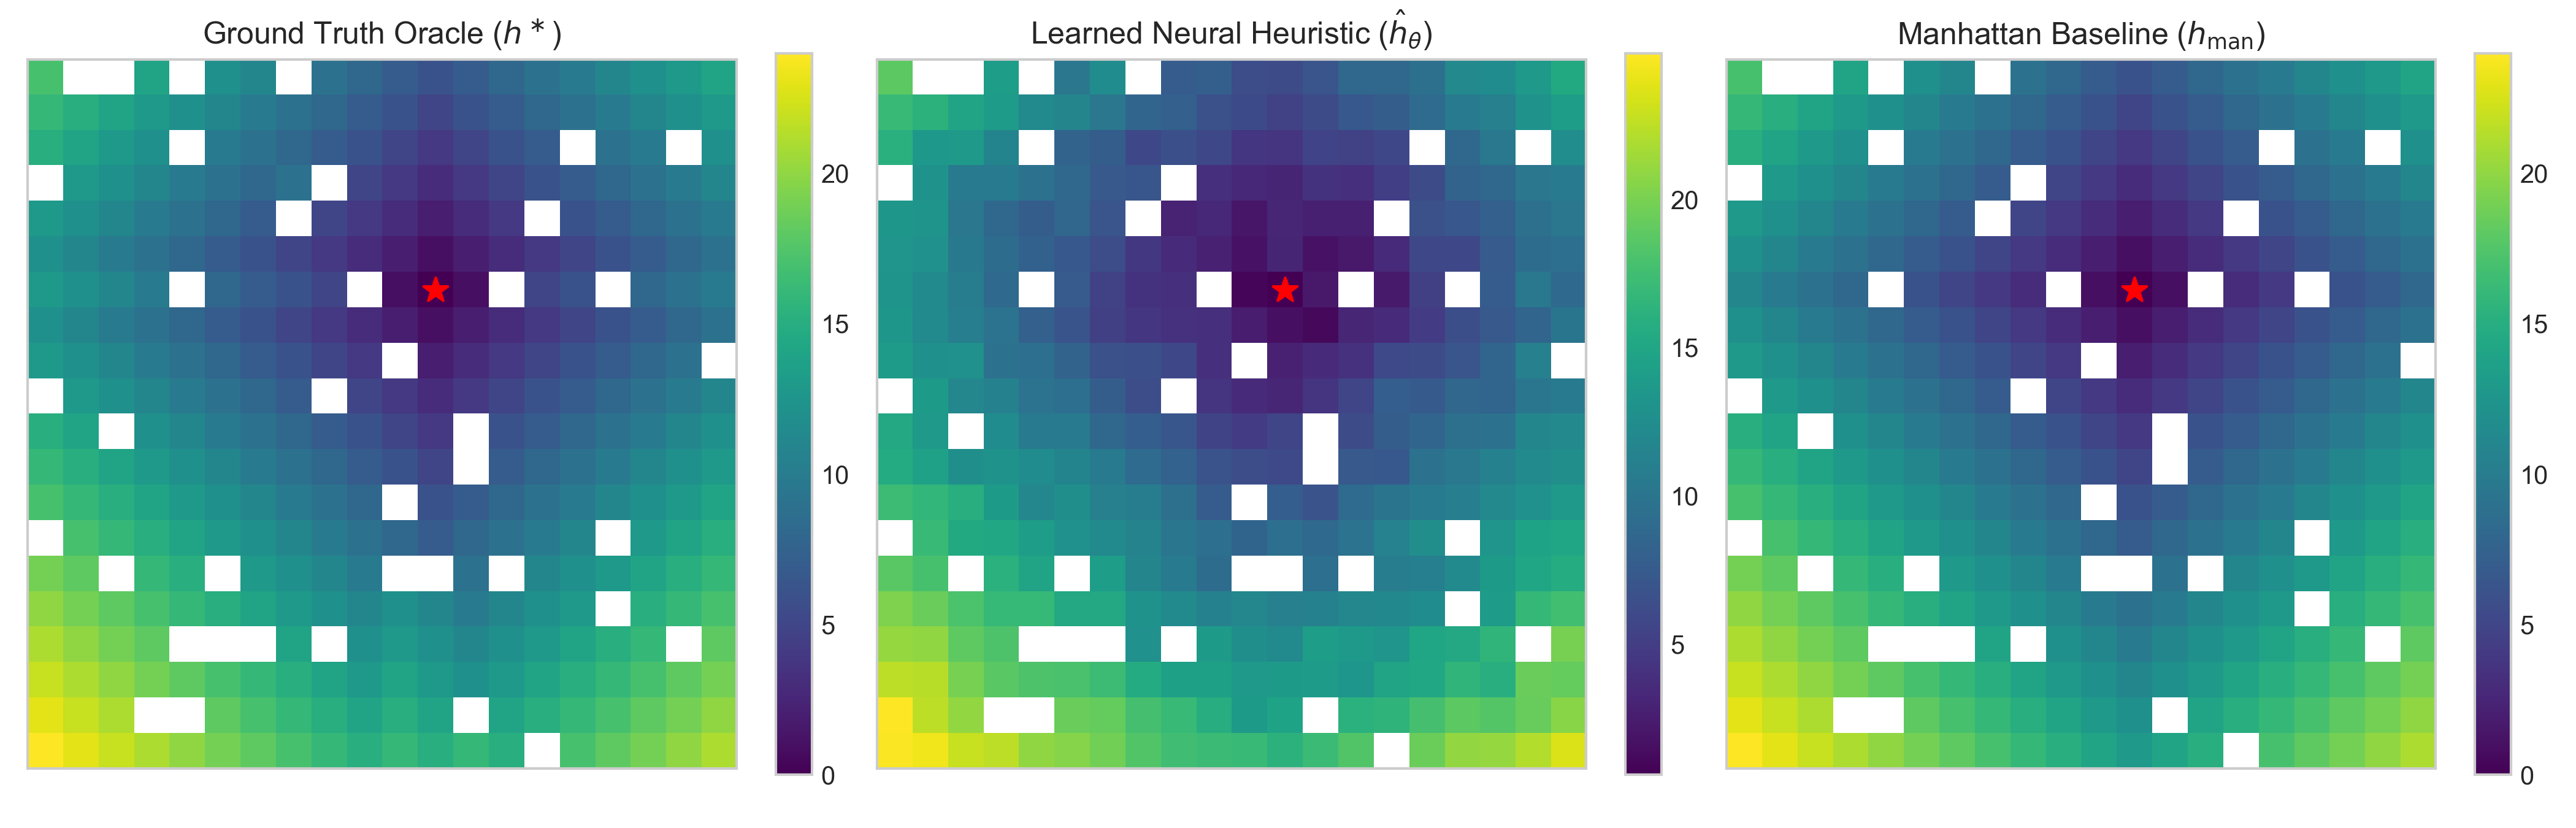
\includegraphics[width=\textwidth]{figures/hstar_vs_prediction_maze.png}
    \caption{Spatial comparison of ground-truth geodesic distance $h^\ast$, predicted neural heuristic $\hat{h}_\theta$, and Manhattan distance $h_{\text{man}}$ from a common goal (red star).}
    \label{fig:heatmaps}
\end{figure}

Whereas Manhattan contour lines remain linear diamonds blind to obstacles, the neural heuristic
curves dynamically around maze corridors and barrier walls, closely approximating the true
geodesic wavefront.

\subsection{Environmental Subgroup Auditing (Bias Analysis)}
Because synthetic grid-mazes do not feature human demographic attributes, algorithmic bias is
formally defined and audited as \emph{environmental and distributional bias} across maze topologies.
Table~\ref{tab:bias_results} reports performance parity across generators, grid dimensions,
obstacle densities, cell positions, and wall clustering.

\begin{table}[H]
\centering
\small
\begin{tabular}{llccccc}
\toprule
\textbf{Subgroup} & \textbf{Partition} & \textbf{MAE (cells)} & \textbf{RMSE (cells)} & \textbf{Signed Err} & \textbf{Inadm. Rate} & \textbf{$\Delta_{\text{expanded}}$ vs Man.} \\
\midrule
Cell Position & Boundary & 4.49 & 8.09 & -0.13 & 60.1\% & --- \\
Cell Position & Interior & 4.33 & 8.67 & -0.81 & 57.4\% & --- \\
Wall Adjacency & Clustered/Adjacent & 5.79 & 9.36 & -0.74 & 56.6\% & --- \\
Wall Adjacency & Open Corridors & 3.95 & 8.19 & -0.53 & 58.8\% & --- \\
Generator & backtracker & --- & --- & --- & --- & -9.0\% \\
Generator & perlin & --- & --- & --- & --- & -4.6\% \\
Grid Size & 20 & --- & --- & --- & --- & 0.2\% \\
Grid Size & 40 & --- & --- & --- & --- & -2.4\% \\
Grid Size & 60 & --- & --- & --- & --- & -9.7\% \\
Grid Size & 80 & --- & --- & --- & --- & -7.0\% \\
Grid Size & 100 & --- & --- & --- & --- & -14.4\% \\
Obstacle Density (%) & 10 & --- & --- & --- & --- & -13.7\% \\
Obstacle Density (%) & 20 & --- & --- & --- & --- & -6.7\% \\
Obstacle Density (%) & 30 & --- & --- & --- & --- & -3.7\% \\
Obstacle Density (%) & 40 & --- & --- & --- & --- & -0.2\% \\
\bottomrule
\end{tabular}
\caption{Environmental and topological subgroup evaluation (Bias and Fairness analysis).}
\label{tab:bias_results}
\end{table}


\begin{figure}[H]
    \centering
    \begin{subfigure}[b]{0.32\textwidth}
        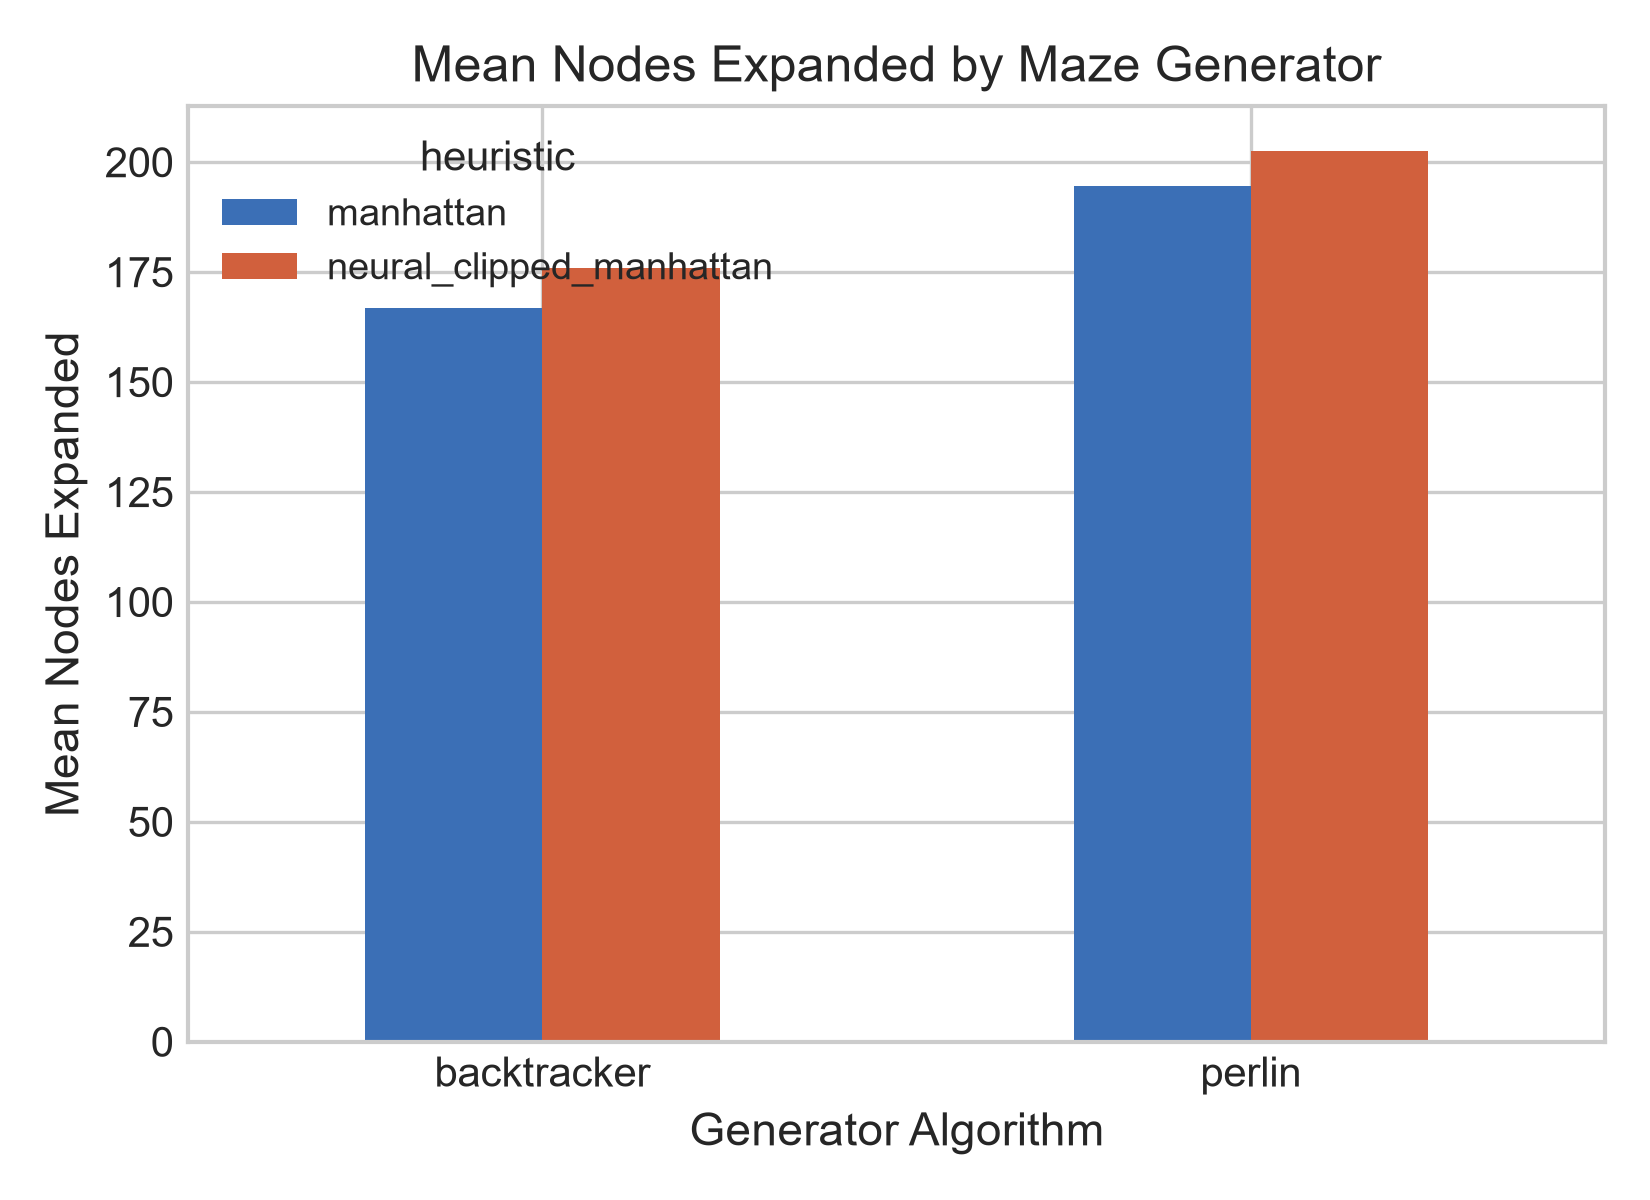
\includegraphics[width=\textwidth]{figures/metrics_by_generator.png}
        \caption{By Generator}
    \end{subfigure}
    \hfill
    \begin{subfigure}[b]{0.32\textwidth}
        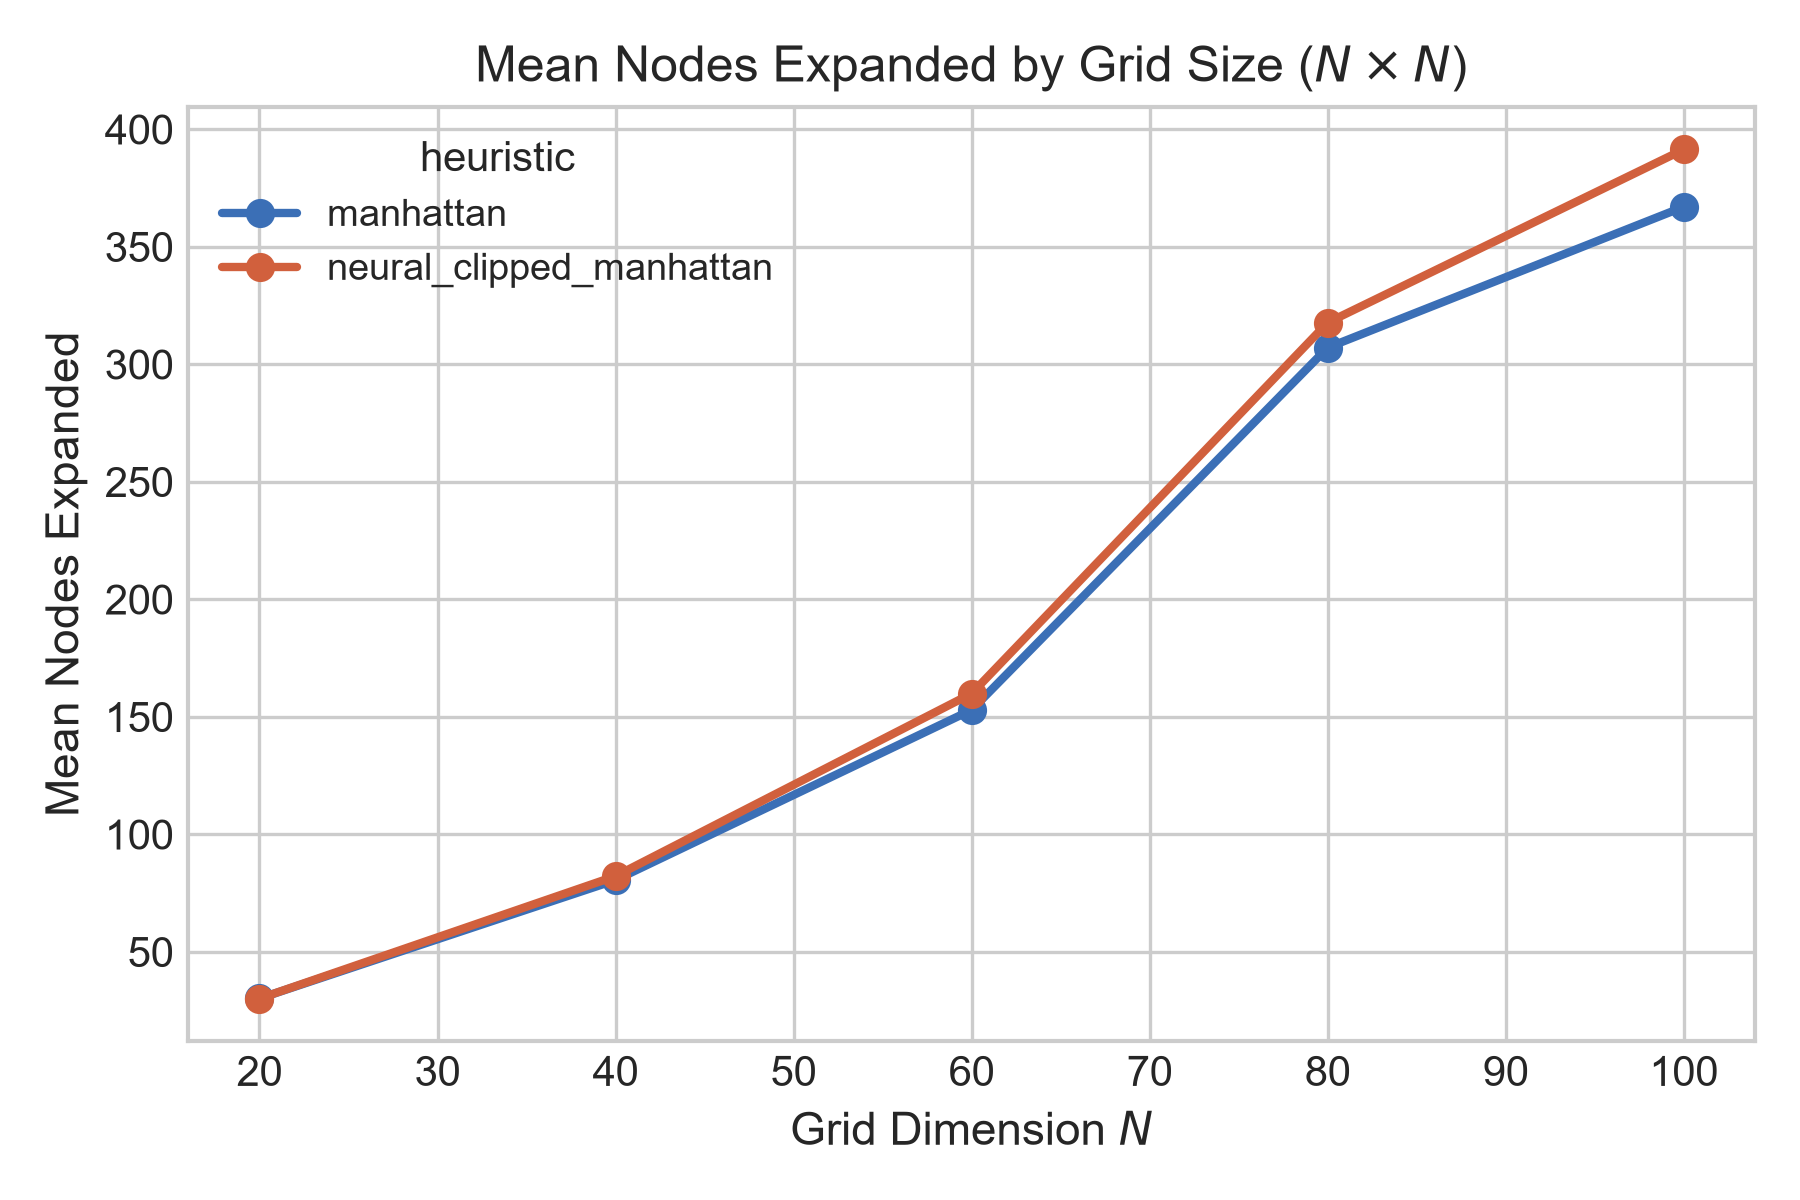
\includegraphics[width=\textwidth]{figures/metrics_by_size.png}
        \caption{By Grid Size ($N$)}
    \end{subfigure}
    \hfill
    \begin{subfigure}[b]{0.32\textwidth}
        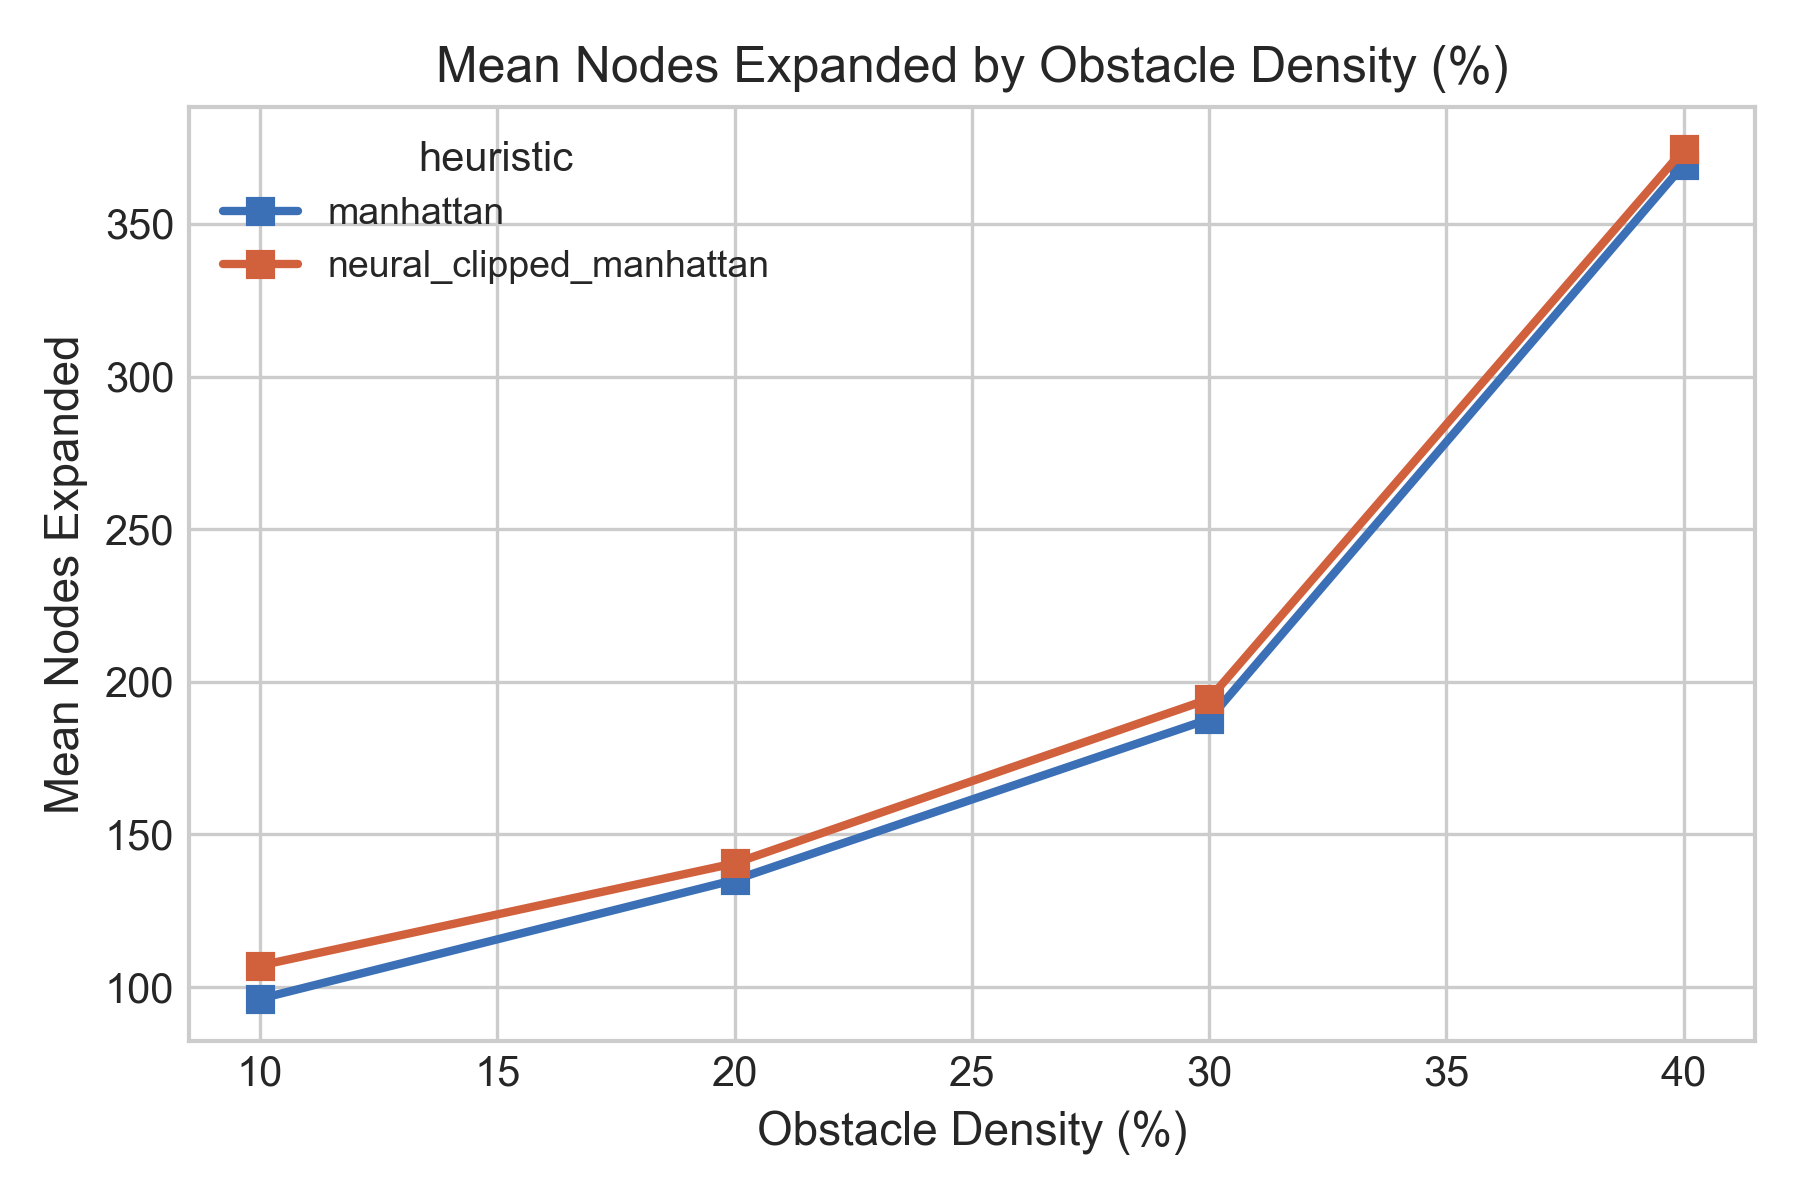
\includegraphics[width=\textwidth]{figures/metrics_by_density.png}
        \caption{By Obstacle Density}
    \end{subfigure}
    \caption{Search node expansion breakdown across environmental subgroups.}
    \label{fig:subgroup_breakdowns}
\end{figure}

Performance remains balanced across both maze generators (backtracker corridors and Perlin noise blobs).
As expected, cell-level errors scale proportionally with grid dimension $N$ because normalized
errors are magnified by grid scale. Crucially, the 100\% success rate is maintained across all
subgroups, demonstrating robust generalizability across diverse topological regimes.
